\documentclass[letterpaper,12pt]{article}

% --- PAQUETES DE IDIOMA
\usepackage[spanish,mexico]{babel}
\usepackage[utf8]{inputenc}
\usepackage{csquotes}

% --- PAQUETES MATEMÁTICOS --
\usepackage{amsmath}
\usepackage{amssymb}
\usepackage{cancel}
\usepackage{mathrsfs}

% --- PAQUETES GRÁFICOS Y DE DISEÑO ---
\usepackage{graphicx}
\usepackage{float}
\usepackage{subcaption}
\usepackage[table]{xcolor}
\usepackage{longtable}
\usepackage{multirow}
\usepackage{makecell}
\usepackage{array}
\usepackage{caption}
\usepackage{tikz}
\usetikzlibrary{decorations.pathmorphing}
\usepackage{circuitikz}
\usetikzlibrary{shapes.geometric, shapes.multipart, shapes.symbols, positioning, arrows.meta, calc, shadows, decorations.pathreplacing,babel}

% --- LISTAS ---
\usepackage{enumitem}

% --- PAQUETES DE CÓDIGO ---
\usepackage{listings}
% Configuración del estilo de listings
\definecolor{codebg}{rgb}{0.95,0.95,0.95}   
\definecolor{keyword}{rgb}{0.0,0.2,0.6}     
\definecolor{comment}{rgb}{0.25,0.5,0.35}   
\definecolor{string}{rgb}{0.6,0.0,0.0}      
\definecolor{number}{rgb}{0.5,0.0,0.5}      
\definecolor{codegray}{rgb}{0.5,0.5,0.5}
\definecolor{codepurple}{rgb}{0.58,0,0.82}
\definecolor{backcolour}{rgb}{0.95,0.95,0.95}

% Definición de los colores utilizados en las tablas
\definecolor{headerbg}{HTML}{5B84C4} % Azul oscuro para el encabezado principal
\definecolor{subheaderbg}{HTML}{B4C6E7} % Azul intermedio para sub-encabezados
\definecolor{rowbg}{HTML}{E9EDF4} % Azul claro para filas intercaladas

\lstset{
  backgroundcolor=\color{backcolour},
  basicstyle=\ttfamily\small,
    inputencoding=utf8,
  keywordstyle=\color{blue}\bfseries,
  stringstyle=\color{codepurple},
  commentstyle=\color{codegray}\itshape,
  numbers=left,
  numberstyle=\tiny\color{codegray},
  frame=single,
  rulecolor=\color{black},
  breaklines=true,
  tabsize=4,
  showstringspaces=false,
  literate={á}{{\'a}}1
           {é}{{\'e}}1
           {í}{{\'i}}1
           {ó}{{\'o}}1
           {ú}{{\'u}}1
           {Á}{{\'A}}1
           {É}{{\'E}}1
           {Í}{{\'I}}1
           {Ó}{{\'O}}1
           {Ú}{{\'U}}1
           {ñ}{{\~n}}1
           {Ñ}{{\~N}}1
           {¿}{{\textquestiondown}}1
           {¡}{{\textexclamdown}}1
           {°}{{\ensuremath{^\circ}}}1
}

% Definición del lenguaje Python para listings
\lstdefinelanguage[LAB]{Python}{
    morekeywords={False, None, True, and, as, assert, async, await, break,
                                class, continue, def, del, elif, else, except, finally,
                                for, from, global, if, import, in, is, lambda, nonlocal,
                                not, or, pass, raise, return, try, while, with, yield,
                                machine, Pin, PWM, ADC, Timer, sleep_ms, sleep_us},
    morecomment=[l]{\#},
    morestring=[b]",
    morestring=[b]',
    sensitive=true
}

% --- ESTILOS PARA DIAGRAMAS DE FLUJO (TIKZ) ---
\tikzset{
  startstop/.style={rectangle, rounded corners, minimum width=3cm, minimum height=1cm,text centered, draw=black, fill=red!30},
  process/.style={rectangle, minimum width=3cm, minimum height=1cm, text centered, draw=black, fill=orange!30},
  decision/.style={diamond, aspect=2, minimum width=3cm, minimum height=1cm, text centered, draw=black, fill=green!30},
  io/.style={trapezium, trapezium left angle=70, trapezium right angle=110, minimum width=3cm, minimum height=1cm, text centered, draw=black, fill=blue!30},
  arrow/.style={thick,->,>=stealth}
}

% Definimos el color dorado/naranja para el cuadro de texto
\definecolor{goldbox}{RGB}{218, 140, 15}

% Macro para dibujar la Raspberry Pi Pico y sus nodos
\newcommand{\picoboard}{
    \draw[thick] (0,0.5) rectangle (4,-9.5);
    \node[align=center, font=\small\sffamily] at (2, -1.5) {Raspberry PI\\[0.1cm]Pico};

    % Pines Superiores
    \draw[red, thick] (0.8, 0.5) -- (0.8, 0.8) coordinate (P41); \node[above, font=\tiny\sffamily, inner sep=1pt] at (P41) {41};
    \draw[red, thick] (2.0, 0.5) -- (2.0, 0.8) coordinate (P42); \node[above, font=\tiny\sffamily, inner sep=1pt] at (P42) {42};
    \draw[red, thick] (3.2, 0.5) -- (3.2, 0.8) coordinate (P43); \node[above, font=\tiny\sffamily, inner sep=1pt] at (P43) {43};
    \node[below, font=\tiny\sffamily] at (0.8, 0.5) {SW CLK};
    \node[below, font=\tiny\sffamily] at (2.0, 0.5) {SW GND};
    \node[below, font=\tiny\sffamily] at (3.2, 0.5) {SW DIO};

    % GND Inferior
    \draw[red, thick] (2, -9.5) -- (2, -10.2) coordinate (PGND);
    \node[above, font=\tiny\sffamily] at (2, -9.5) {GND};
    \node[below, font=\tiny\sffamily] at (2, -10.2) {3,8,13,18 \quad 23,28,38};

    % Pines del lado Izquierdo
    \foreach \i/\pin/\num in {
        1/GP0/1, 2/GP1/2, 
        4/GP2/4, 5/GP3/5, 6/GP4/6, 7/GP5/7, 
        9/GP6/9, 10/GP7/10, 11/GP8/11, 12/GP9/12, 
        14/GP10/14, 15/GP11/15, 16/GP12/16, 17/GP13/17, 
        19/GP14/19, 20/GP15/20
    } {
        \draw[red, thick] (0, -\i*0.45) -- (-0.4, -\i*0.45) coordinate (P\num);
        \node[right, font=\tiny\sffamily] at (0, -\i*0.45) {\pin};
        \node[above left, font=\tiny\sffamily, inner sep=1pt] at (P\num) {\num};
    }

    % Pines del lado Derecho
    \foreach \i/\pin/\num in {
        1/VBUS/40, 2/VSS/39, 
        4/3V3\_EN/37, 5/3V3/36, 6/ADC\_VREF/35, 7/GP28\_A2/34, 8/AGND/33, 
        9/GP27\_A1/32, 10/GP26\_A0/31, 11/RUN/30, 12/GP22/29, 
        14/GP21/27, 15/GP20/26, 16/GP19/25, 17/GP18/24, 
        19/GP17/22, 20/GP16/21
    } {
        \draw[red, thick] (4, -\i*0.45) -- (4.4, -\i*0.45) coordinate (P\num);
        \node[left, font=\tiny\sffamily] at (4, -\i*0.45) {\pin};
        \node[above right, font=\tiny\sffamily, inner sep=1pt] at (P\num) {\num};
    }
}



\definecolor{azulresultado}{HTML}{0072C6}
\definecolor{rojoacarreo}{HTML}{FF0000}

% Colores para la tabla
\definecolor{headblue}{HTML}{4F81BD}
\definecolor{subheadblue}{HTML}{B8CCE4}
\definecolor{datablockblue}{HTML}{DCE6F1}

% --- RUTAS DE IMÁGENES ---
\graphicspath{{img/}{portada_img/}}

\definecolor{armblue}{RGB}{0, 113, 188}

% --- CONFIGURACIÓN DE PÁGINA (GEOMETRÍA) ---
\usepackage[
    left=25mm, 
    right=25mm,
    top=35mm,
    bottom=30mm,
    headheight=77pt, 
    papersize={21.59cm,27.94cm}
]{geometry}

% --- FORMATO DE TEXTO ---
\renewcommand{\baselinestretch}{1.25} 
\usepackage{parskip} 
\usepackage{lipsum}  

% --- VARIABLES GLOBALES ---
\newcommand{\materia}{}

% --- ENCABEZADOS Y PIES DE PÁGINA ---
\usepackage{fancyhdr}
\pagestyle{fancy}
\fancyhf{} 
\fancyhead[L]{
\includegraphics[height=1.5cm]{portada_img/izq.png}}
\fancyhead[R]{
\includegraphics[height=1.5cm]{portada_img/der.png}}
\fancyfoot[C]{\thepage} 
\renewcommand{\headrulewidth}{0.4pt} 
\renewcommand{\footrulewidth}{0pt}  

% --- BIBLIOGRAFÍA ---
\usepackage[backend=biber, style=apa, sortcites, url=true]{biblatex}
\addbibresource{referencias.bib}

% --- HIPERVÍNCULOS ---
\usepackage{hyperref}
\hypersetup{
    colorlinks=true,
    linkcolor=blue,
    citecolor=blue,
    filecolor=magenta,
    urlcolor=cyan
}

\begin{document}

    \input{portada.tex}

    \newpage
    \setcounter{page}{1}

    \section{Objetivo:}
    
    Conocer el funcionamiento del ADC (convertidor analógico digital) para realizar aplicaciones que requieran procesar señales en el mundo continuo, convertir señales provenientes de sensores; aprender el funcionamiento del control PWM.
    
   \section*{Actividad 1}
Comentar el siguiente programa, e indicar que hace:

\lstinputlisting[language={[LAB]Python}, caption=Figura 6.3. Código de prueba, basicstyle=\ttfamily\scriptsize]{Code/Ac1SinNombres.py}

\subsection*{Propuesta de solución}
El programa implementa la lectura del sensor de temperatura interno del microcontrolador RP2040 y utiliza un convertidor analógico-digital (ADC). El  sensor de temperatura está conectado internamente al canal 4 del ADC, permitiendo medir la temperatura del chip sin necesidad de componentes externos.

Para lograr esta actividad primero se configura el ADC en el canal 4 mediante la clase \texttt{ADC(4)}. Dentro de un bucle infinito, se realiza la lectura del valor bruto de 16 bits (0 a 65535) que representa el voltaje proporcional a la temperatura. Este valor se convierte a voltaje real mediante la fórmula \texttt{Valor * (3.3 / 65535)}. Posteriormente, se aplica la ecuación oficial del fabricante para transformar el voltaje en grados Celsius: 
\[
T = 27 - \frac{V - 0.706}{0.001721}
\]
Finalmente, se imprime la temperatura y se aplica un retardo de 1 segundo para evitar saturar la salida serial y tener una visualización cómoda de las lecturas.

\begin{center}
\begin{tikzpicture}[node distance=1.8cm, scale=0.78, transform shape, every node/.style={font=\small}]
    \node (start) [startstop] {Inicio};
    
    \node (import) [process, below=1cm of start] 
    {Importar \texttt{ADC}, \texttt{Pin}, \texttt{time}};
    
    \node (config) [process, below=1cm of import, text width=4.5cm] 
    {Configurar ADC canal 4\\ (sensor de temperatura interno)};
    
    \node (read) [process, below=1cm of config, text width=4.5cm] 
    {Leer ADC y convertir a voltaje:\\ $Valor = lectura \times (3.3 / 65535)$};
    
    \node (temp) [process, below=1cm of read, text width=4.5cm] 
    {Calcular temperatura:\\ $Temp = 27 - (Valor - 0.706) / 0.001721$};
    
    \node (print) [process, below=1cm of temp] 
    {Imprimir temperatura};
    
    \node (delay) [process, below=1cm of print] 
    {Esperar 1 segundo};
    
    % Flechas
    \draw [arrow] (start) -- (import);
    \draw [arrow] (import) -- (config);
    \draw [arrow] (config) -- (read);
    \draw [arrow] (read) -- (temp);
    \draw [arrow] (temp) -- (print);
    \draw [arrow] (print) -- (delay);
    
    % Loop infinito
    \draw [arrow] (delay) -- ++(4.0 cm,0) |- (read.east);

\end{tikzpicture}
\end{center}

El flujo de datos comienza importando los módulos necesarios y configurando el ADC en el canal 4, que internamente está conectado al sensor de temperatura del RP2040. Dentro del bucle infinito, se lee el valor bruto de 16 bits del ADC, el cual representa la señal analógica convertida a digital. Este valor se convierte a voltaje real mediante una regla de tres simple, considerando que el ADC tiene un rango de 0 a 65535 para 0 a 3.3V.

Una vez obtenido el voltaje, se aplica la ecuación característica del sensor de temperatura proporcionada por el fabricante (Raspberry Pi), que establece una relación lineal entre voltaje y temperatura. El resultado se imprime en la consola de Thonny y se espera 1 segundo antes de repetir el ciclo, permitiendo una visualización ordenada y evitando saturar el buffer de salida.

\subsection*{Desarrollo}

\lstinputlisting[language={[LAB]Python}, caption=Código de la Actividad 1, basicstyle=\ttfamily\scriptsize]{Code/Act1.py}

\begin{figure}[H]
    \centering
    
\includegraphics[width=0.8\textwidth]{img/Actividad1/Act1_1.jpg}
    \caption{Lecturas iniciales del sensor de temperatura. Se observan valores estables alrededor de 26.1°C a 27.9°C.}
    \label{fig:act1_1}
\end{figure}

\begin{figure}[H]
    \centering
    
\includegraphics[width=0.8\textwidth]{img/Actividad1/Act1_2.jpg}
    \caption{Continuidad de lecturas tras varios ciclos. La lectura se mantiene estable.}
    \label{fig:act1_2}
\end{figure}

\begin{figure}[H]
    \centering
    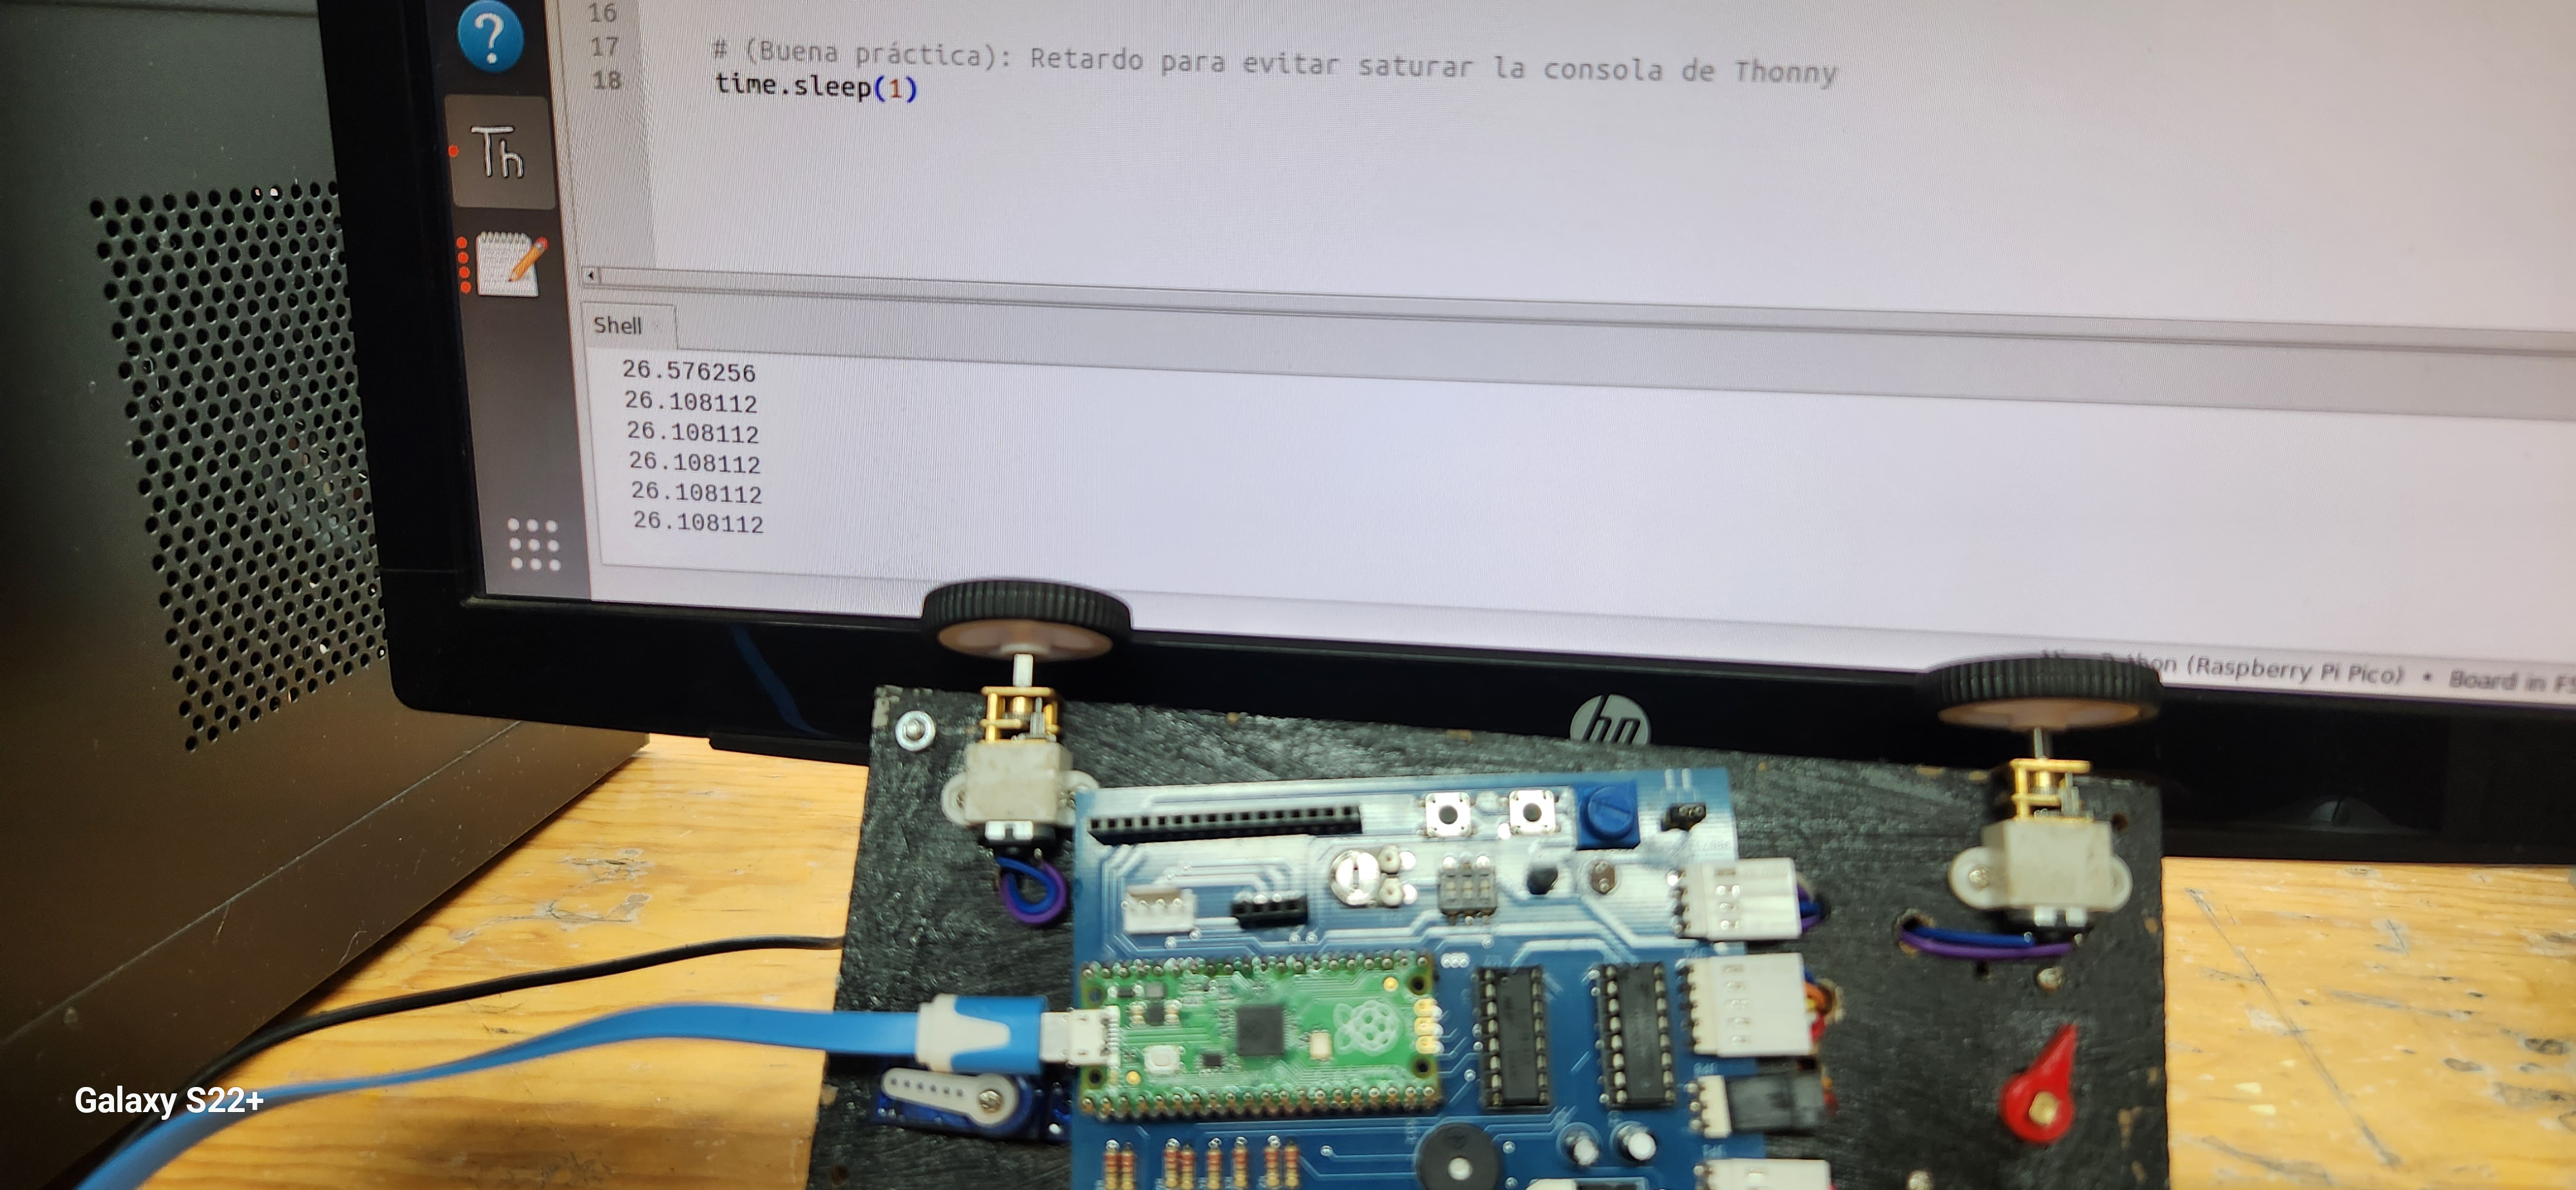
\includegraphics[width=0.8\textwidth]{img/Actividad1/Act1_3.jpg}
    \caption{Lecturas posteriores mostrando pequeñas variaciones.}
    \label{fig:act1_3}
\end{figure}

\subsection*{Análisis de resultados}

El programa cumple con el objetivo de leer y mostrar la temperatura interna del RP2040 mediante su ADC interno. Las lecturas obtenidas (26.1°C a 27.9°C) son consistentes con la temperatura normal del chip. La conversión de valor bruto a voltaje y la aplicación de la ecuación del fabricante permiten obtener temperaturas con precisión aceptable y las pequeñas variaciones entre lecturas son normales debido a la actividad del procesador y condiciones ambientales. Esto fue posible gracias al uso del ADC interno, la aplicación de fórmulas de calibración y la implementación de bucles con retardos para adquisición periódica de datos.

    
    \section*{Actividad 2}

Realizar un programa que despliegue en la consola de Thonny el resultado de la conversión y el voltaje generado por el potenciómetro; actualizar cada segundo.

\begin{figure}[htbp]
    \centering
    % Se mantiene la escala y transform shape
    \begin{tikzpicture}[>=latex, scale=0.9, transform shape]

        % 1. Dibujar la Raspberry Pi Pico (esto se mantiene igual)
        \picoboard

        % 2. Conexiones del Potenciómetro (Moveremos la columna X principal)
        % Nueva coordenada X principal para la columna del potenciómetro: 6.2 (antes 5.2)

        % Línea verde de señal al pin GP26_A0 (P31). Se extiende a la nueva X=6.2
        \draw[green!70!black, thick] (P31) -- (6.2, -4.5);
        \fill[green!70!black] (6.2, -4.5) circle (1.5pt); % Nodo de conexión superior

        % Línea roja a 3.3V (se mueve a X=6.2)
        \draw[red, thick] (6.2, -4.5) -- (6.2, -3.5);
        
        % Símbolo de 3.3V (se mueve y se ajusta el centrado a X=6.2)
        \draw[thick] (5.9, -3.5) -- (6.5, -3.5); % Antes 4.9 a 5.5
        \node[above, font=\sffamily] at (6.2, -3.5) {3.3V};

        % Símbolo de resistencia del potenciómetro (zigzag) (se mueve a X=6.2)
        \draw[thick, decoration={zigzag, segment length=3.5mm, amplitude=1.5mm}, decorate] (6.2, -4.5) -- (6.2, -6.5);

        % Línea roja a Tierra (GND) (se mueve a X=6.2)
        \draw[red, thick] (6.2, -6.5) -- (6.2, -7.5);
        
        % Símbolo de Tierra (GND) (se mueve y se ajusta el centrado a X=6.2)
        \draw[thick] (5.8, -7.5) -- (6.6, -7.5); % Antes 4.8 a 5.6
        \draw[thick] (5.95, -7.65) -- (6.45, -7.65); % Antes 4.95 a 5.45
        \draw[thick] (6.1, -7.8) -- (6.3, -7.8); % Antes 5.1 a 5.3
        \draw[thick] (6.18, -7.95) -- (6.22, -7.95); % Antes 5.18 a 5.22

        % Flecha y etiqueta del potenciómetro (se mueven)
        % La flecha sale de la nueva X=6.2 y va a X=7.2 (antes 6.2)
        \draw[->, thick] (6.2, -5.5) -- (7.2, -6.2);
        \node[right, font=\sffamily, align=left] at (7.2, -6.2) {Potenciómetro\\10k$\Omega$};

        % Pequeños números indicadores de pin (grises) (se mueven a la izquierda de la nueva X=6.2)
        \node[left, font=\tiny\sffamily, text=gray] at (6.1, -4.3) {3};
        \node[left, font=\tiny\sffamily, text=gray] at (6.1, -4.7) {1};
        \node[left, font=\tiny\sffamily, text=gray] at (6.1, -6.3) {2};

        % 3. Cuadro Amarillo de Conversión (También se mueve para evitar solapamiento)
        % Se ajustó la posición (anchor=west) a X=6.5 (antes 5.5) para mantener la separación
        \node[draw=goldbox, thick, text=goldbox, align=left, font=\sffamily\large\bfseries, inner sep=6pt, fill=white, anchor=west] 
        at (6.5, -1.5) {Conversión = 65535 ; Voltaje = 3.30 Volts\\[0.1cm]Conversión = 0 ; Voltaje = 0 Volts};

        % 4. Título de la figura en la parte inferior (se mantiene igual)
        \node[font=\sffamily\Large] at (3.5, -11.5) {Figura 6-4. Circuito y ejecución; actividad 2};

    \end{tikzpicture}
\end{figure}


\subsection*{Propuesta de solución}

El programa implementa la lectura de un potenciómetro conectado al pin analógico GPIO26 (ADC0) de la Raspberry Pi Pico. Utiliza el convertidor analógico-digital (ADC) interno del RP2040 para obtener un valor digital de 16 bits (0 a 65535) proporcional al voltaje aplicado en la entrada analógica y este valor lo convertimos posteriormente a voltaje real en el rango de 0 a 3.3 V mediante una regla de tres. Para lograrolo, primero se configura el ADC en el pin GPIO26 mediante la clase \texttt{ADC(26)}. Dentro de un bucle infinito, se realiza la lectura del valor bruto de 16 bits mediante el método \texttt{read\_u16()}. Este valor se convierte a voltaje real aplicando la fórmula:

\[
V = \text{lectura} \times \frac{3.3}{65535}
\]

Finalmente, se imprime en la terminal de thony el valor de conversión como el voltaje calculado con dos decimales, y se espera 1 segundo antes de repetir el ciclo para una visualización ordenada y evitando saturar la salida serial.

El diagrama de flujo a continuación ilustra el proceso:

\begin{center}
\begin{tikzpicture}[node distance=1.8cm, scale=0.78, transform shape, every node/.style={font=\small}]
    \node (start) [startstop] {Inicio};
    
    \node (import) [process, below=1cm of start] 
    {Importar \texttt{ADC}, \texttt{time}};
    
    \node (config) [process, below=1cm of import, text width=4.5cm] 
    {Configurar ADC en pin GPIO26 (ADC0)};
    
    \node (read) [process, below=1cm of config, text width=4.5cm] 
    {Leer ADC con \texttt{read\_u16()} \\ \texttt{conversion = valor digital (0-65535)}};
    
    \node (volt) [process, below=1cm of read, text width=4.5cm] 
    {Calcular voltaje:\\ \texttt{voltaje = conversion * (3.3 / 65535)}};
    
    \node (print) [process, below=1cm of volt] 
    {Imprimir: \texttt{conversion} y \texttt{voltaje}};
    
    \node (delay) [process, below=1cm of print] 
    {Esperar 1 segundo};
    
    % Flechas
    \draw [arrow] (start) -- (import);
    \draw [arrow] (import) -- (config);
    \draw [arrow] (config) -- (read);
    \draw [arrow] (read) -- (volt);
    \draw [arrow] (volt) -- (print);
    \draw [arrow] (print) -- (delay);
    
    % Loop infinito
    \draw [arrow] (delay) -- ++(4.0 cm,0) |- (read.east);

\end{tikzpicture}
\end{center}

El flujo de datos comienza importando los módulos necesarios y configurando el ADC en el pin GPIO26, que corresponde al canal 0 del convertidor analógico-digital y dentro del bucle infinito, se lee el valor bruto de 16 bits del ADC, el cual representa la señal analógica del potenciómetro convertida a digital. Este valor se convierte a voltaje real mediante una regla de tres simple, considerando que el ADC tiene un rango de 0 a 65535 para 0 a 3.3 V. El resultado se imprime en la consola de Thonny con el formato solicitado y se espera 1 segundo antes de repetir el ciclo.

\subsection*{Desarrollo}

\lstinputlisting[language={[LAB]Python}, caption=Código de la Actividad 2, basicstyle=\ttfamily\scriptsize]{Code/Act2.py}

\begin{figure}[H]
    \centering
    
\includegraphics[width=0.8\textwidth]{img/Actividad2/Act2_1.jpg}
    \caption{Lecturas iniciales con el potenciómetro en una posición fija intermedia. Se observan valores estables alrededor de 1.78 V.}
    \label{fig:act2_1}
\end{figure}

\begin{figure}[H]
    \centering
    
\includegraphics[width=0.8\textwidth]{img/Actividad2/Act2_2.jpg}
    \caption{Lecturas al variar el potenciómetro. Se observa un aumento progresivo hasta alcanzar el máximo de 3.30 V.}
    \label{fig:act2_2}
\end{figure}

\begin{figure}[H]
    \centering
    
\includegraphics[width=0.8\textwidth]{img/Actividad2/Act2_3.jpg}
    \caption{Continuidad de lecturas cerca del máximo. Se muestran valores cercanos a 3.30 V con ligeras variaciones.}
    \label{fig:act2_3}
\end{figure}

\begin{figure}[H]
    \centering
    
\includegraphics[width=0.8\textwidth]{img/Actividad2/Act2_4.jpg}
    \caption{Sr varia el potenciometro y los valores bajan a a lrededor de 1.85 V.}
    \label{fig:act2_4}
\end{figure}

\begin{figure}[H]
    \centering
    
\includegraphics[width=0.8\textwidth]{img/Actividad2/Act2_5.jpg}
    \caption{Lecturas finales al reducir el voltaje hasta valores bajos cercanos a 0.88 V.}
    \label{fig:act2_5}
\end{figure}

\subsection*{Análisis de resultados}

El programa cumple con el objetivo de leer el potenciómetro y mostrar el valor de conversión y voltaje en consola. En la Figura \ref{fig:act2_1} se observan lecturas estables en posición intermedia (35352-35409, 1.78 V), demostrando la estabilidad del ADC y al variar el potenciómetro (Figura \ref{fig:act2_2}), el valor aumenta progresivamente hasta 65535 (3.30 V), con una transición suave y lineal que confirma la correcta relación resistencia-voltaje. Las Figuras \ref{fig:act2_3}, \ref{fig:act2_4} y \ref{fig:act2_5} muestran lecturas consistentes en distintas posiciones: máximo, intermedio y bajo y la conversión de 16 bits ofrece buena precisión y el retardo de 1 segundo permite una visualización clara en consola.

\section*{Actividad 3}

Empleando el divisor de voltaje generado por la foto-resistencia; tomar la lectura de voltaje, registrar el máximo y mínimo obtenido, fijar un valor de referencia. Mientras la lectura es menor a la referencia, mantenga en bajo el GPIO7 y cuando sobrepase el valor configurado lo ponga en alto.

\begin{figure}[htbp]
    \centering
    \begin{tikzpicture}[>=latex, scale=0.85, transform shape]

        % 1. Dibujar la Raspberry Pi Pico
        \picoboard

        % 2. Conexiones del Divisor de Voltaje
        \draw[green!70!black, thick] (P32) -- (6.2, -4.05);
        \fill[green!70!black] (6.2, -4.05) circle (1.5pt);

        % --- Foto-resistencia ---
        \draw[red, thick] (6.2, -4.05) -- (6.2, -3.0);
        \draw[thick, rounded corners=8pt] (5.8, -3.0) rectangle (6.6, -1.5);
        \draw[thick, rounded corners=2pt] (6.2, -3.0) -- (6.2, -2.8) 
                    -- (5.9, -2.8) -- (5.9, -2.55) 
                    -- (6.5, -2.55) -- (6.5, -2.3)
                    -- (5.9, -2.3) -- (5.9, -2.05)
                    -- (6.5, -2.05) -- (6.5, -1.8)
                    -- (6.2, -1.8) -- (6.2, -1.5);
        \draw[red, thick] (6.2, -1.5) -- (6.2, -0.5);
        \node[right, font=\sffamily] at (6.6, -2.25) {Fotoresistencia};
        \draw[thick] (5.9, -0.5) -- (6.5, -0.5);
        \node[above, font=\sffamily] at (6.2, -0.5) {3.3V};

        \node[left, font=\tiny\sffamily, text=gray] at (6.1, -1.0) {2};
        \node[left, font=\tiny\sffamily, text=gray] at (6.1, -3.5) {1};

        % --- Resistencia R1 ---
        \draw[green!70!black, thick] (6.2, -4.05) -- (6.2, -4.5);
        \draw[thick, decoration={zigzag, segment length=3.5mm, amplitude=1.5mm}, decorate] (6.2, -4.5) -- (6.2, -6.0);
        \draw[red, thick] (6.2, -6.0) -- (6.2, -6.5);
        \node[right, font=\sffamily, align=left] at (6.5, -5.25) {R1\\10k$\Omega$};
        
        \draw[thick] (5.8, -6.5) -- (6.6, -6.5);
        \draw[thick] (5.95, -6.65) -- (6.45, -6.65);
        \draw[thick] (6.1, -6.8) -- (6.3, -6.8);

        \node[left, font=\tiny\sffamily, text=gray] at (6.1, -4.3) {2};
        \node[left, font=\tiny\sffamily, text=gray] at (6.1, -6.2) {1};

        % 3. Elementos de Lectura (Lado Derecho)
        % Desplazados hacia la derecha para no encimarse con "Fotoresistencia"
        \node[draw=goldbox, thick, text=goldbox, font=\sffamily\Large\bfseries, inner sep=5pt, anchor=west] 
        at (8.5, -1) {Lectura de la foto-resistencia:};

        \node[anchor=west, font=\sffamily\Large\bfseries] at (9.8, -2.5) {V\textsubscript{MIN} =};
        \draw[gray, thick] (11.8, -2.6) -- (17.5, -2.6);

        \node[anchor=west, font=\sffamily\Large\bfseries] at (9.8, -3.5) {V\textsubscript{MAX} =};
        \draw[gray, thick] (11.8, -3.6) -- (17.5, -3.6);

        \node[anchor=west, font=\sffamily\Large\bfseries] at (9.8, -4.5) {V\textsubscript{REF} =};
        \draw[gray, thick] (11.8, -4.6) -- (17.5, -4.6);

        % 4. Tabla de Condiciones Inferior
        \fill[goldbox!20] (7.5, -6.6) rectangle (17.5, -7.4);
        
        \draw[goldbox, thick] (7.5, -5.8) rectangle (17.5, -7.4); 
        \draw[goldbox, thick] (7.5, -6.6) -- (17.5, -6.6); 
        \draw[goldbox, thick] (12.5, -5.8) -- (12.5, -7.4); 

        % Textos de la tabla (Fila 1) 
        \node[text=goldbox, font=\sffamily\normalsize\bfseries] at (10.0, -6.2) {V\textsubscript{Foto\_resistencia} $<$ V\textsubscript{REF}};
        \node[text=goldbox, font=\sffamily\normalsize\bfseries] at (15.0, -6.2) {V\textsubscript{Foto\_resistencia} $>$ V\textsubscript{REF}};

        % Textos de la tabla (Fila 2)
        \node[text=goldbox, font=\sffamily\Large\bfseries] at (10.0, -7.0) {GPIO7 = '0'};
        \node[text=goldbox, font=\sffamily\Large\bfseries] at (15.0, -7.0) {GPIO7 = '1'};

        % 5. Título de la figura en la parte inferior
        \node[font=\sffamily\Large] at (7.5, -11.5) {Figura 6-5. Circuito de foto-resistencia; actividad 3};

    \end{tikzpicture}
\end{figure}

\newpage

\subsection*{Propuesta de solución}

El programa implementa un sistema de control de iluminación basado en una fotoresistencia (LDR) conectada al pin analógico GPIO27 (ADC1) de la Raspberry Pi Pico. La fotoresistencia forma un divisor de voltaje junto con una resistencia fija de 10 k$\Omega$, generando un voltaje variable que depende de la cantidad de luz incidente y este voltaje se convierte a un valor digital de 16 bits o de 0 a 65535 mediante el convertidor analógico-digital (ADC) interno como en activiades pasadas.

Para conseguir implementar lo solicitado, primero se configura el ADC en el pin GPIO27 mediante la clase \texttt{ADC(27)} y se configura el pin GPIO7 como salida digital para controlar un LED, además se definen otras variables para almacenar los valores máximo y mínimo históricos de luz, así como un valor de referencia (umbral) que determina cuándo se debe encender el LED. Dentro de un bucle infinito, se realiza la lectura del valor digital de la fotoresistencia, se actualizan los valores máximo y mínimo si es necesario, y se compara la lectura actual con el umbral: si la lectura supera el umbral, se enciende el LED; en caso contrario, se apaga.

El diagrama de flujo a continuación ilustra el proceso:

\begin{center}
\begin{tikzpicture}[node distance=1.8cm, scale=0.78, transform shape, every node/.style={font=\small}]
    \node (start) [startstop] {Inicio};
    
    \node (import) [process, below=1cm of start] 
    {Importar \texttt{ADC}, \texttt{Pin}, \texttt{time}};
    
    \node (config) [process, below=1cm of import, text width=4.5cm] 
    {Configurar ADC en GPIO27\\ Configurar GPIO7 como salida};
    
    \node (vars) [process, below=1cm of config, text width=4.5cm] 
    {Inicializar: \texttt{V\_REF = 30000}\\ \texttt{val\_max = 0}\\ \texttt{val\_min = 65535}};
    
    \node (read) [process, below=1cm of vars, text width=4.5cm] 
    {Leer ADC: \texttt{lectura = read\_u16()}};
    
    \node (update) [process, below=1cm of read, text width=4.5cm] 
    {Actualizar \texttt{val\_max} y \texttt{val\_min}};
    
    \node (compare) [decision, below=1cm of update, text width=3cm] 
    {¿\texttt{lectura > V\_REF}?};
    
    \node (led_on) [process, below=1cm of compare, text width=2.5cm, yshift=-0.5cm] 
    {LED = 1\\ (Encendido)};
    
    \node (led_off) [process, below=1cm of compare, text width=2.5cm, yshift=-0.5cm] 
    {LED = 0\\ (Apagado)};
    
    \node (print) [process, below=2cm of led_on, text width=5cm] 
    {Imprimir: \texttt{lectura}, \texttt{val\_min}, \texttt{val\_max}, \texttt{V\_REF}};
    
    \node (delay) [process, below=1cm of print] 
    {Esperar 0.5 segundos};
    
    % Flechas
    \draw [arrow] (start) -- (import);
    \draw [arrow] (import) -- (config);
    \draw [arrow] (config) -- (vars);
    \draw [arrow] (vars) -- (read);
    \draw [arrow] (read) -- (update);
    \draw [arrow] (update) -- (compare);
    
    \draw [arrow] (compare) -- node[anchor=west] {Sí} (led_on);
    \draw [arrow] (compare) -- node[anchor=east] {No} (led_off);
    
    \draw [arrow] (led_on) -- (print);
    \draw [arrow] (led_off) -- (print);
    \draw [arrow] (print) -- (delay);
    
    % Loop infinito
    \draw [arrow] (delay) -- ++(4.0 cm,0) |- (read.east);

\end{tikzpicture}
\end{center}

El flujo de datos comienza importando los módulos necesarios y configurando los pines correspondientes: el GPIO27 como entrada analógica para la fotoresistencia y el GPIO7 como salida digital para controlar el LED. Dentro del bucle infinito, se lee el valor analógico de la fotoresistencia, se actualizan los valores máximos y mínimos históricos, y se compara la lectura actual con el umbral predefinido. Esta comparación determina el estado del LED, que se enciende cuando hay suficiente luz (lectura mayor al umbral) y se apaga cuando la luz es insuficiente. Los resultados se muestran en consola cada 0.5 segundos.

\subsection*{Desarrollo}

\lstinputlisting[language={[LAB]Python}, caption=Código de la Actividad 3, basicstyle=\ttfamily\scriptsize]{Code/Act3.py}

\begin{figure}[H]
    \centering
    
\includegraphics[width=0.8\textwidth]{img/Actividad3/Act3_1.jpg}
    \caption{Lecturas iniciales con luz ambiental constante. Se observan valores estables alrededor de 38800-39353 y como son mayores que el valor umbral el led se mantiene en alto (encendido).}
    \label{fig:act3_1}
\end{figure}

\begin{figure}[H]
    \centering
    
\includegraphics[width=0.8\textwidth]{img/Actividad3/Act3_2.jpg}
    \caption{Al tapar la fotoresistencia se disminuye drasticamente el valor máximo de la iluminación pasando de 7569 a 2688 lo que provoca la desactivación del LED.}
    \label{fig:act3_2}
\end{figure}

\begin{figure}[H]
    \centering
    
\includegraphics[width=0.8\textwidth]{img/Actividad3/Act3_3.jpg}
    \caption{Al retirar la mano y aumentar drasticamente la iluminación a 398097 el Led vuelve a encenderse.}
    \label{fig:act3_3}
\end{figure}

\begin{figure}[H]
    \centering
    
\includegraphics[width=0.8\textwidth]{img/Actividad3/Act3_4.jpg}
    \caption{Por último al tapar una vez más la fotorrsistencia vuelve a haber un cambio drástico en la iluminación (4833)por lo que el led vuelve a apagarse.}
    \label{fig:act3_4}
\end{figure}

\subsection*{Análisis de resultados}

El programa logra ek objetivo de controlar el estado del LED en función de la cantidad de luz que incide sobre la fotoresistencia. En la Figura \ref{fig:act3_1} se observan lecturas estables con luz ambiental constante, donde los valores de conversión se mantienen alrededor de 38800-39353. Al ser estos valores superiores al umbral establecido, el LED permanece encendido, demostrando la correcta configuración inicial del sistema. En la Figura \ref{fig:act3_2}, al tapar la fotoresistencia, el valor de iluminación disminuye drásticamente desde 7569 hasta 2688, lo que provoca que la lectura quede por debajo del umbral y, por tanto, el LED se desactive. Esta respuesta evidencia la sensibilidad del sensor y la eficacia de la lógica de control implementada.

Al retirar la mano (Figura \ref{fig:act3_3}), la iluminación aumenta de manera abrupta alcanzando un valor de 398097, superando nuevamente el umbral y provocando que el LED se encienda y finalmente, en la Figura \ref{fig:act3_4}, al tapar una vez más la fotoresistencia, el valor desciende a 4833, ubicándose por debajo del umbral y apagando el LED nuevamente. En todos los casos, el sistema responde de forma inmediata y consistente ante los cambios en las condiciones de iluminación, validando el correcto funcionamiento del ADC, la actualización de los valores máximo y mínimo, y la lógica de comparación con el umbral de referencia.


    \newpage
    \section*{Actividad 4}

    Realizar un programa que muestre el valor de temperatura tanto en C como en F, en la consola de Thonny del sensor interno y del sensor TMP36; indicando cual de ellos tiene valor mayor al otro.

    \begin{figure}[htbp]
        \centering
        \begin{tikzpicture}[>=latex, scale=0.85, transform shape]

            % 1. Dibujar la Raspberry Pi Pico
            \picoboard

            % 2. Sensor TMP36
            % Etiqueta superior (movida más arriba para no encimarse con 3.3V)
            \node[font=\sffamily] at (6.5, 0.6) {Sensor de temperatura};

            % Caja del sensor
            \draw[thick] (5.5, -4.5) rectangle (7.5, -1.2);
            \node[font=\sffamily] at (6.5, -1.6) {TMP36};

            % Pin VCC (Derecha superior)
            \node[left, font=\tiny\sffamily] at (7.5, -2.2) {VCC};
            \node[right, font=\tiny\sffamily, text=gray] at (7.5, -2.2) {1};

            % Pin VOUT (Izquierda, hacia P34 que es GP28_A2)
            \node[right, font=\tiny\sffamily] at (5.5, -3.15) {VOUT};
            \node[left, font=\tiny\sffamily, text=gray] at (5.5, -3.15) {2};

            % Conexión P34 a VOUT (línea recta horizontal)
            \draw[green!70!black, thick] (P34) -- (5.5, -3.15);
            \fill[green!70!black] (5.5, -3.15) circle (1.5pt); % Nodo de conexión verde

            % Conexión VCC a 3.3V
            \draw[green!70!black, thick] (7.5, -2.2) -- (8.5, -2.2) -- (8.5, -0.5);
            \draw[thick] (8.1, -0.5) -- (8.9, -0.5); % Línea horizontal de 3.3V
            \node[above, font=\sffamily] at (8.5, -0.5) {3.3V};

            % Pin GND (Derecha inferior)
            \node[left, font=\tiny\sffamily] at (7.5, -3.9) {GND};
            \node[right, font=\tiny\sffamily, text=gray] at (7.5, -3.9) {3};

            % Conexión GND a Tierra
            \draw[red, thick] (7.5, -3.9) -- (8.5, -3.9) -- (8.5, -5.0);

            % Símbolo de Tierra (GND)
            \draw[thick] (8.1, -5.0) -- (8.9, -5.0);
            \draw[thick] (8.25, -5.15) -- (8.75, -5.15);
            \draw[thick] (8.4, -5.3) -- (8.6, -5.3);

            % 3. Bloque de Texto Lateral (reducido para que no se salga de la hoja)
            % Línea superior
            \draw[thick] (9.5, -1.5) -- (17.5, -1.5);

            % Textos (con fuente más pequeña)
            \node[anchor=west, font=\sffamily\normalsize] at (9.5, -2.1) {Temperatura interna = 19$^\circ$C; 66$^\circ$F};
            \node[anchor=west, font=\sffamily\normalsize] at (9.5, -2.7) {Temperatura externa TMP36 = 20$^\circ$C; 68$^\circ$F};
            \node[anchor=west, font=\sffamily\normalsize] at (9.5, -3.3) {El sensor TMP36 tiene el valor mayor};
            \node[anchor=west, font=\sffamily\normalsize] at (9.5, -3.9) {de temperatura};

            % Línea inferior
            \draw[thick] (9.5, -4.4) -- (17.5, -4.4);

            % 4. Título de la figura (movido más abajo)
            \node[font=\sffamily\Large] at (8.5, -11.2) {Figura 6-6. Circuito sensor TMP36 y sensor interno; actividad 4};

        \end{tikzpicture}
    \end{figure}

    \subsection*{Propuesta de solución}

    Para obtener y comparar las lecturas de temperatura, se propone utilizar los convertidores analógico-digitales (ADC) del microcontrolador. Se inicializan dos instancias de la clase \texttt{ADC}: el canal 4, reservado internamente en el RP2040 para medir la temperatura del dado de silicio, y el canal asignado al \texttt{GPIO28} para leer el voltaje analógico del sensor externo TMP36. 
    
    Dentro de un bucle continuo, el procesador lee los registros de 16 bits de ambos ADC y los escala al voltaje de referencia del sistema (3.3V). A partir de estos voltajes, se aplican las ecuaciones de transferencia específicas de cada sensor para obtener los grados Celsius. Posteriormente, se realiza una conversión matemática simple a grados Fahrenheit. Finalmente, se implementa una estructura de control \texttt{if-elif-else} que evalúa y compara aritméticamente ambos resultados para imprimir en la consola serial las magnitudes exactas y el veredicto de cuál sensor registra la mayor temperatura, introduciendo un retardo de 2 segundos entre cada muestreo.


    \begin{figure}[htbp]
        \centering
        \begin{tikzpicture}[>=latex, scale=0.65, transform shape,
            inicio/.style={ellipse, draw, thick, minimum width=2.2cm, minimum height=0.9cm, fill=green!20},
            proceso/.style={rectangle, draw, thick, minimum width=3.2cm, minimum height=0.9cm, fill=blue!10, align=center, font=\small},
            decision/.style={diamond, draw, thick, minimum width=1.8cm, minimum height=1.2cm, fill=yellow!20, align=center, aspect=2, font=\small},
            flecha/.style={->, thick}
        ]
            % Inicio
            \node[inicio] (inicio) at (0, 0) {Inicio};

            % Configuración
            \node[proceso] (config) at (0, -1.8) {Configurar ADC(4) y ADC(28)};

            % Lectura sensor interno
            \node[proceso] (leer_int) at (0, -3.6) {Leer voltaje sensor interno};

            % Calcular temp interna
            \node[proceso] (calc_int) at (0, -5.4) {Calcular temp\_c\_int};

            % Lectura TMP36
            \node[proceso] (leer_tmp) at (0, -7.2) {Leer voltaje sensor TMP36};

            % Calcular temp TMP36
            \node[proceso] (calc_tmp) at (0, -9) {Calcular temp\_c\_tmp};

            % Imprimir temperaturas
            \node[proceso] (imprimir) at (0, -10.8) {Imprimir temperaturas};

            % Decisión 1
            \node[decision] (dec1) at (0, -13.2) {temp\_c\_int $>$\\temp\_c\_tmp?};

            % Imprimir interno mayor
            \node[proceso] (msg_int) at (-5.5, -13.2) {Sensor interno\\es mayor};

            % Decisión 2
            \node[decision] (dec2) at (5.5, -13.2) {temp\_c\_tmp $>$\\temp\_c\_int?};

            % Imprimir TMP36 mayor
            \node[proceso] (msg_tmp) at (5.5, -16.5) {TMP36 es\\mayor};

            % Imprimir iguales
            \node[proceso] (msg_igual) at (10.5, -13.2) {Temperaturas\\iguales};

            % Esperar
            \node[proceso] (esperar) at (0, -19) {Esperar 2 segundos};

            % Flechas principales
            \draw[flecha] (inicio) -- (config);
            \draw[flecha] (config) -- (leer_int);
            \draw[flecha] (leer_int) -- (calc_int);
            \draw[flecha] (calc_int) -- (leer_tmp);
            \draw[flecha] (leer_tmp) -- (calc_tmp);
            \draw[flecha] (calc_tmp) -- (imprimir);
            \draw[flecha] (imprimir) -- (dec1);

            % Decisión 1 - Sí (izquierda)
            \draw[flecha] (dec1.west) -- node[above] {Sí} (msg_int.east);
            \draw[flecha] (msg_int.south) -- (-5.5, -19) -- (esperar.west);

            % Decisión 1 - No (derecha)
            \draw[flecha] (dec1.east) -- node[above] {No} (dec2.west);

            % Decisión 2 - Sí (abajo)
            \draw[flecha] (dec2.south) -- node[right] {Sí} (msg_tmp.north);
            \draw[flecha] (msg_tmp.south) -- (5.5, -19) -- (esperar.east);

            % Decisión 2 - No (derecha)
            \draw[flecha] (dec2.east) -- node[above] {No} (msg_igual.west);
            \draw[flecha] (msg_igual.south) -- (10.5, -19) -- (5.5, -19);

            % Loop de regreso
            \draw[flecha] (esperar.south) -- (0, -20.5) -- (-8, -20.5) -- (-8, -3.6) -- (leer_int.west);

        \end{tikzpicture}
        \caption{Diagrama de flujo del código de la Actividad 4}
    \end{figure}

    El diagrama de flujo muestra el proceso de lectura y comparación de dos sensores de temperatura. Primero, se configuran los convertidores analógico-digitales ADC(4) para el sensor interno de la Raspberry Pi Pico y ADC(28) para el sensor externo TMP36. Dentro de un ciclo infinito, se lee el voltaje del sensor interno, se convierte a grados Celsius y Fahrenheit, y luego se repite el mismo proceso para el sensor TMP36. Después de imprimir ambas temperaturas en consola, el programa evalúa mediante decisiones condicionales cuál sensor reporta una temperatura mayor: si el sensor interno es mayor se imprime ese mensaje, si el TMP36 es mayor se indica así, y si ambos son iguales se muestra que las temperaturas coinciden. Finalmente, el programa espera 2 segundos antes de repetir todo el ciclo.


    \subsection*{Desarrollo}

    \lstinputlisting[language={[LAB]Python}, caption=Código de la Actividad 4, basicstyle=\ttfamily\scriptsize]{Code/Act4.py}

    \begin{figure}[H]
        \centering
        
\includegraphics[width=0.85\textwidth]{img/Actividad4/Act4_2.jpg}
        \caption{Estado inicial de las lecturas. El sensor interno del microcontrolador registra una temperatura estable de 26.1 °C. A su vez, la lectura de voltaje en el GPIO28 (simulando el TMP36) se calcula en 25.7 °C. El programa compara ambas variables numéricas y la terminal muestra correctamente que el sensor interno tiene el valor mayor.}
    \end{figure}

    \begin{figure}[H]
        \centering
        
\includegraphics[width=0.85\textwidth]{img/Actividad4/Act4_4.jpg}
        \caption{Actualización dinámica en tiempo real. Al aumentar físicamente el voltaje de entrada en el pin analógico, el ADC detecta el cambio al instante. El código procesa el nuevo nivel eléctrico, obteniendo 28.5 °C para el TMP36. El bloque condicional reacciona a este incremento y actualiza la consola indicando el cambio de estado a favor del sensor externo.}
    \end{figure}

    \begin{figure}[H]
        \centering
        
\includegraphics[width=0.85\textwidth]{img/Actividad4/Act4_5.jpg}
        \caption{Transición a la baja. Se disminuye el voltaje inyectado al convertidor analógico, lo que hace que la temperatura calculada para el TMP36 caiga a 25.2 °C. El ciclo de muestreo capta este descenso y la terminal refleja la corrección, devolviendo el veredicto lógico al sensor interno de forma automática.}
    \end{figure}

    \begin{figure}[H]
        \centering
        
\includegraphics[width=0.85\textwidth]{img/Actividad4/Act4_6.jpg}
        \caption{Seguimiento continuo y estabilidad. Al elevar nuevamente la señal analógica, la lectura simulada alcanza un pico de 29.7 °C, superando de nuevo a los 26.1 °C fijos del encapsulado. Esto comprueba que ambos canales del convertidor operan de forma aislada e independiente, permitiendo un monitoreo cruzado confiable cada 2 segundos.}
    \end{figure}

    \subsection*{Análisis de resultados}

    La ejecución del código muestra claramente la capacidad del microcontrolador para medir señales analógicas continuas. La instrucción \texttt{read\_u16()} captura la conversión del ADC; aunque el hardware del RP2040 tiene una resolución nativa de 12 bits, MicroPython la escala automáticamente a 16 bits, entregando un valor discreto entre 0 y 65535. Al multiplicar este valor por \texttt{(3.3 / 65535)}, se recupera el nivel de voltaje analógico real presente en los pines.

    Para el sensor interno, la lectura del voltaje (\texttt{v\_int}) se procesa a través de la ecuación típica de la polarización directa de su diodo, donde un voltaje de 0.706V equivale a 27°C, con una pendiente negativa de 1.721mV por grado. En contraste, la señal del sensor externo TMP36 (\texttt{v\_tmp}) tiene una respuesta completamente lineal y positiva. A este voltaje se le resta un \textit{offset} de 0.5V (necesario en el sensor para poder leer temperaturas bajo cero) y se multiplica por 100, de acuerdo con su sensibilidad física de 10mV/°C. 

    El bloque condicional actúa como un comparador lógico digital. Al procesar las variables flotantes \texttt{temp\_c\_int} y \texttt{temp\_c\_tmp}, el flujo del programa se dirige con éxito hacia la instrucción \texttt{print} correspondiente. Esto comprueba que el sistema no solo realiza la lectura y el ajuste de la señal eléctrica, sino que también es capaz de tomar decisiones por software basándose en cambios físicos en tiempo real.


    \newpage

    \section*{Actividad 5}

    Escribir el siguiente programa, comentar e indicar que hace:

    \lstinputlisting[language={[LAB]Python}, caption=Código; actividad 5, basicstyle=\ttfamily\scriptsize]{Code/Act5SinNombre.py}

    \subsection*{Propuesta de solución}
    El programa tiene como objetivo generar un incremento gradual en la potencia entregada a una carga (típicamente un LED) utilizando Modulación por Ancho de Pulso (PWM). La solución consiste en configurar el \texttt{GPIO1} como un canal PWM y fijar su frecuencia en 1 kHz. En lugar de encender el pin de manera directa (todo o nada), se emplea un ciclo \texttt{for} para recorrer el registro del ciclo de trabajo (\textit{duty cycle}) desde 0 hasta su límite de 16 bits (65535), avanzando en incrementos de 500 unidades. Se introduce un pequeño retardo de 50 milisegundos en cada paso para que el incremento de luz sea fácil de notar a simple vista. Al terminar el ciclo, la señal PWM se apaga por completo durante 2 segundos antes de volver a empezar.

    \begin{figure}[htbp]
        \centering
        \begin{tikzpicture}[>=latex, scale=0.8, transform shape,
            inicio/.style={ellipse, draw, thick, minimum width=2cm, minimum height=0.8cm, fill=green!20},
            proceso/.style={rectangle, draw, thick, minimum width=3cm, minimum height=0.7cm, fill=blue!10, align=center, font=\footnotesize},
            decision/.style={diamond, draw, thick, minimum width=1.5cm, minimum height=1cm, fill=yellow!20, align=center, aspect=2, font=\footnotesize},
            flecha/.style={->, thick}
        ]
            % Inicio
            \node[inicio] (inicio) at (0, 0) {Inicio};

            % Configurar PWM
            \node[proceso] (config_pwm) at (0, -1.4) {Configurar PWM en GPIO1};

            % Establecer frecuencia
            \node[proceso] (freq) at (0, -2.8) {Frecuencia = 1000 Hz};

            % Inicializar duty
            \node[proceso] (init_duty) at (0, -4.2) {duty = 0};

            % Decisión del for
            \node[decision] (dec_for) at (0, -6) {duty $<$ 65535?};

            % Aplicar PWM (a la derecha)
            \node[proceso] (aplicar) at (5, -6) {pwm.duty\_u16(duty)};

            % Esperar 0.05s
            \node[proceso] (esperar1) at (5, -7.6) {Esperar 0.05 s};

            % Incrementar duty
            \node[proceso] (incrementar) at (5, -9.2) {duty = duty + 500};

            % Apagar PWM (abajo de la decisión)
            \node[proceso] (apagar) at (0, -8.2) {pwm.duty\_u16(0)};

            % Esperar 2s
            \node[proceso] (esperar2) at (0, -9.8) {Esperar 2 segundos};

            % Flechas principales
            \draw[flecha] (inicio) -- (config_pwm);
            \draw[flecha] (config_pwm) -- (freq);
            \draw[flecha] (freq) -- (init_duty);
            \draw[flecha] (init_duty) -- (dec_for);

            % Decisión - Sí (entra al for, hacia la derecha)
            \draw[flecha] (dec_for.east) -- node[above] {Sí} (aplicar.west);
            \draw[flecha] (aplicar) -- (esperar1);
            \draw[flecha] (esperar1) -- (incrementar);
            % Loop del for regresa arriba
            \draw[flecha] (incrementar.east) -- (7.5, -9.2) -- (7.5, -4.8) -- (0, -4.8) -- (dec_for.north);

            % Decisión - No (sale del for, hacia abajo)
            \draw[flecha] (dec_for.south) -- node[left] {No} (apagar.north);
            \draw[flecha] (apagar) -- (esperar2);

            % Loop de regreso al while (por la izquierda)
            \draw[flecha] (esperar2.south) -- (0, -11) -- (-3.5, -11) -- (-3.5, -4.2) -- (init_duty.west);

        \end{tikzpicture}
        \caption{Diagrama de flujo del código de la Actividad 5}
    \end{figure}

    El diagrama de flujo representa el control de un LED mediante modulación por ancho de pulso (PWM). El programa inicia configurando el pin GPIO1 como salida PWM y estableciendo una frecuencia de 1000 Hz. Dentro de un ciclo infinito (while), se inicializa la variable duty en 0 y comienza un ciclo for que incrementa gradualmente el ciclo de trabajo. En cada iteración del ciclo for, se verifica si duty es menor a 65535 (valor máximo de 16 bits); si es así, se aplica el valor de duty al PWM, se espera 0.05 segundos y se incrementa duty en 500 unidades, creando un efecto de aumento gradual de brillo en el LED. Cuando duty alcanza o supera 65535, el ciclo for termina, se apaga el PWM estableciendo duty en 0, y el programa espera 2 segundos antes de reiniciar todo el proceso, generando un efecto de respiración continuo en el LED.


    \subsection*{Desarrollo}

    \lstinputlisting[language={[LAB]Python}, caption=Código de la Actividad 5 Comentado,basicstyle=\ttfamily\scriptsize]{Code/Act5.py}

    \begin{figure}[H]
        \centering
        
\includegraphics[width=0.8\textwidth]{img/Actividad5/Act5_4.jpg}
        \caption{Estado de reposo. El registro del ciclo de trabajo se encuentra en cero (\texttt{pwm.duty\_u16(0)}), por lo que el pin GPIO1 no entrega voltaje y el LED se mantiene apagado. Este estado representa tanto el punto de partida del programa como la pausa de 2 segundos programada al final del bucle principal.}
    \end{figure}

    \begin{figure}[H]
        \centering
        
\includegraphics[width=0.8\textwidth]{img/Actividad5/Act5_3.jpg}
        \caption{Inicio del incremento gradual (\textit{fade-in}). Al entrar al ciclo \texttt{for}, el valor de la variable de trabajo comienza a subir. En esta etapa temprana, el ancho de los pulsos activos es corto, entregando un voltaje promedio bajo a la salida que hace que el LED se ilumine de forma muy tenue.}
    \end{figure}

    \begin{figure}[H]
        \centering
        
\includegraphics[width=0.7\textwidth]{img/Actividad5/Act5_1.jpg}
        \caption{Pico máximo de iluminación. El contador del ciclo se acerca a su límite de 16 bits (65535). En este punto, la señal PWM permanece en nivel alto la mayor parte de su periodo de 1 milisegundo. Esto suministra el voltaje eficaz máximo (cercano a 3.3V) a la carga, haciendo que el LED alcance su brillo total justo antes de cortarse la señal para reiniciar el proceso.}
    \end{figure}

    \subsection*{Análisis de resultados}

    El script muestra el uso de temporizadores por hardware para controlar el voltaje promedio de salida. La instrucción \texttt{PWM(Pin(1))} asocia el terminal físico a un bloque PWM interno, mientras que \texttt{pwm.freq(1000)} establece el periodo de la onda en exactamente 1 milisegundo. Como esta frecuencia es mucho más rápida que lo que el ojo humano puede captar, cualquier LED conectado no se verá parpadeando, sino como una luz fija.

    El ciclo iterativo modifica de forma constante la anchura del pulso activo. La instrucción \texttt{pwm.duty\_u16(duty)} inserta el valor actual del contador en el registro del PWM. Cuando la variable \texttt{duty} vale 0, el pin se mantiene en 0V todo el tiempo. Conforme el ciclo \texttt{for} avanza en pasos de 500, el tiempo que el pin pasa en 3.3V se va alargando poco a poco. Físicamente, esto provoca un aumento gradual del voltaje eficaz (RMS) que llega al componente, creando el conocido efecto visual de encendido suave o "respiración" (\textit{fade-in}) en el LED.

    Finalmente, la instrucción \texttt{pwm.duty\_u16(0)} fuera del ciclo regresa el registro a cero, cortando de inmediato el voltaje de salida. El retardo de \texttt{time.sleep(2)} detiene el programa principal, manteniendo el LED apagado por dos segundos completos. Esto deja claro cómo se pueden combinar de manera sencilla las rutinas de control continuo en segundo plano (como el PWM) con pausas directas en el flujo de ejecución.

    \newpage

    \section*{Actividad 6}
    Modificar el programa para que incremente y decremente de manera automática el valor de PWM en la terminal GPIO0 y refleje el valor inverso en el pin GPIO1.

    \begin{figure}[htbp]
        \centering
        \begin{tikzpicture}[>=latex, scale=0.8, transform shape]

            % 1. Dibujar la Raspberry Pi Pico
            \picoboard

            % ==========================================
            % 2. CIRCUITO (Izquierda - Separados y con LEDs hacia abajo)
            % ==========================================

            % --- Rama GP0 (Pin 1 - Verde, la más alejada a la izquierda) ---
            \draw[green!70!black, thick] (P1) -- (-3.0, -0.45);
            \node[above, font=\tiny\sffamily, text=gray] at (-0.8, -0.45) {1};
            \node[above, font=\tiny\sffamily, text=gray] at (-2.8, -0.45) {2};
            
            % Resistencia Superior
            \draw[thick, decoration={zigzag, segment length=3.5mm, amplitude=1.5mm}, decorate] (-3.0, -0.45) -- (-4.5, -0.45);
            \node[above, font=\sffamily] at (-3.75, -0.2) {220$\Omega$};
            \node[above, font=\tiny\sffamily, text=gray] at (-4.7, -0.45) {1};

            % Doblez hacia abajo (Columna X = -5.0)
            \draw[green!70!black, thick] (-4.5, -0.45) -- (-5.0, -0.45) -- (-5.0, -1.2);
            \node[left, font=\tiny\sffamily, text=gray] at (-5.0, -1.0) {1};
            
            % LED 1 (Triángulo apuntando hacia ABAJO)
            \draw[thick] (-5.3, -1.2) -- (-4.7, -1.2) -- (-5.0, -1.8) -- cycle; % Triángulo
            \draw[thick] (-5.3, -1.8) -- (-4.7, -1.8); % Línea base (cátodo)
            
            % Flechas de luz apuntando hacia abajo-izquierda
            \draw[thick, -latex] (-5.4, -1.3) -- (-5.7, -1.7);
            \draw[thick, -latex] (-5.25, -1.45) -- (-5.55, -1.85);
            
            \node[left, font=\tiny\sffamily, text=gray] at (-5.0, -2.0) {2};

            % Conexión a Tierra 1
            \draw[green!70!black, thick] (-5.0, -1.8) -- (-5.0, -2.5);
            \draw[thick] (-5.4, -2.5) -- (-4.6, -2.5);
            \draw[thick] (-5.25, -2.65) -- (-4.75, -2.65);
            \draw[thick] (-5.1, -2.8) -- (-4.9, -2.8);


            % --- Rama GP1 (Pin 2 - Rojo, la más cercana a la Pico) ---
            \draw[red, thick] (P2) -- (-1.5, -0.9);
            \node[above, font=\tiny\sffamily, text=gray] at (-0.8, -0.9) {2};
            \node[above, font=\tiny\sffamily, text=gray] at (-1.3, -0.9) {2};

            % Resistencia Inferior
            \draw[thick, decoration={zigzag, segment length=3.5mm, amplitude=1.5mm}, decorate] (-1.5, -0.9) -- (-3.0, -0.9);
            \node[above, font=\sffamily] at (-2.25, -1.8) {220$\Omega$};
            \node[above, font=\tiny\sffamily, text=gray] at (-3.2, -0.9) {1};
            
            % Doblez hacia abajo (Columna X = -3.5)
            \draw[red, thick] (-3.0, -0.9) -- (-3.5, -0.9) -- (-3.5, -1.2);
            \node[left, font=\tiny\sffamily, text=gray] at (-3.5, -1.05) {1};

            % LED 2 (Triángulo apuntando hacia ABAJO)
            \draw[thick] (-3.8, -1.2) -- (-3.2, -1.2) -- (-3.5, -1.8) -- cycle; % Triángulo
            \draw[thick] (-3.8, -1.8) -- (-3.2, -1.8); % Línea base (cátodo)
            
            % Flechas de luz apuntando hacia abajo-izquierda
            \draw[thick, -latex] (-3.9, -1.3) -- (-4.2, -1.7);
            \draw[thick, -latex] (-3.75, -1.45) -- (-4.05, -1.85);

            \node[left, font=\tiny\sffamily, text=gray] at (-3.5, -2.0) {2};

            % Conexión a Tierra 2
            \draw[green!70!black, thick] (-3.5, -1.8) -- (-3.5, -2.5);
            \draw[thick] (-3.9, -2.5) -- (-3.1, -2.5);
            \draw[thick] (-3.75, -2.65) -- (-3.25, -2.65);
            \draw[thick] (-3.6, -2.8) -- (-3.4, -2.8);

            % ==========================================
            % 3. OSCILOGRAMAS (Derecha)
            % ==========================================
            
            \node[anchor=west, font=\sffamily\Large\bfseries] at (5.5, -2.5) {GPIO0};
            
            \begin{scope}[shift={(7.5, -2.5)}]
                \draw[thick] (0, 0.4) -- ++(0.5, 0); 
                \foreach \x/\w in {0.5/0.2, 0.9/0.2, 1.3/0.2, 1.7/0.2, 2.1/0.2, 2.5/0.2, 2.9/0.2, 3.3/0.2, 3.7/0.2, 4.1/0.2, 4.5/0.2, 4.9/0.2, 5.3/0.2} {
                    \draw[thick] (\x, 0.4) -- (\x, 0) -- ++(\w, 0) -- ++(0, 0.4) -- ++(0.2, 0);
                }
                \draw[thick] (5.9, 0.4) -- ++(0.1, 0);
            \end{scope}

            \node[anchor=west, font=\sffamily\Large\bfseries] at (5.5, -4.5) {GPIO1};
            
            \begin{scope}[shift={(7.5, -4.5)}]
                \draw[thick] (0, 0) -- ++(1.0, 0); 
                \foreach \x/\w in {1.0/0.8, 2.8/0.8, 4.6/0.8} {
                    \draw[thick] (\x, 0) -- (\x, 0.4) -- ++(\w, 0) -- ++(0, -0.4) -- ++(1.0, 0);
                }
                \draw[thick] (6.4, 0) -- ++(0.1, 0);
            \end{scope}

            % ==========================================
            % 4. TÍTULO DE LA FIGURA
            % ==========================================
            \node[font=\sffamily\Large] at (4.0, -11.0) {Figura 6-8. Circuito y oscilograma requerido; actividad 6};

        \end{tikzpicture}
    \end{figure}

    \subsection*{Propuesta de solución}

    Para poder implementar las modificaciones que se solicitan en la actividad, deben realizar las implementaciones de incrementar y decrementar automáticamente el valor PWM, que esto sea en la terminal \texttt{GPIO0} y reflejar el valor inverso en el pin \texttt{GPIO1}. 

    Para poder realizar esa implementación, es necesario configurar ambos pines como salidas PWM, para esto se crean dos objetos de la clase \texttt{PWM} independientes que se asocian a cada pin. Luego, se establece la misma frecuencia de 1 kHz para ambos canales.

    Posteriormente se establecen los limites, ya que el ciclo de trabajo de un PWM en MicroPython se controla mediante un registro de 16 bits, lo que implica que los valores válidos van de 0 a 65535, el valor máximo se guarda en la constante \texttt{MAX\_DUTY}, adicionalmente se define un variable \texttt{PASO} con valor de \texttt{1000} esto hace que el incremento o decremento del ciclo de trabajo sea de 1000 unidades, lo que permite observar claramente el cambio en la intensidad del LED conectado a cada pin.

    Posteriormente, se implementa un bucle infinito que contiene dos ciclos \texttt{for} anidados. El primer ciclo incrementa el valor de \texttt{duty} desde 0 hasta el valor máximo, aplicando el mismo valor a \texttt{pwm0} y el valor inverso a \texttt{pwm1}. Luego, el segundo ciclo hace lo contrario, decrementando el valor de \texttt{duty} desde el máximo hasta 0, manteniendo la relación inversa entre ambos canales. Se introduce un retardo de 20 milisegundos en cada iteración para que los cambios sean perceptibles visualmente.

\begin{figure}[htbp]
    \centering
    \begin{tikzpicture}[>=latex, scale=0.75, transform shape,
        inicio/.style={ellipse, draw, thick, minimum width=2cm, minimum height=0.8cm, fill=green!20},
        proceso/.style={rectangle, draw, thick, minimum width=3cm, minimum height=0.7cm, fill=blue!10, align=center, font=\footnotesize},
        decision/.style={diamond, draw, thick, minimum width=1.5cm, minimum height=1cm, fill=yellow!20, align=center, aspect=2, font=\footnotesize},
        flecha/.style={->, thick, rounded corners=2pt} % Esquinas redondeadas para mayor fluidez
    ]
        % Inicio
        \node[inicio] (inicio) at (0, 0) {Inicio};

        % Configurar PWM
        \node[proceso] (config_pwm) at (0, -1.4) {Configurar PWM0 en GPIO0\\Configurar PWM1 en GPIO1};

        % Establecer variables iniciales
        \node[proceso] (vars) at (0, -3) {freq = 1000 Hz\\MAX\_DUTY = 65535\\PASO = 1000};

        % ---------------- FASE 1 ----------------
        % Inicializar duty Fase 1
        \node[proceso] (init_duty1) at (0, -4.8) {duty = 0};

        % Decisión del primer for
        \node[decision] (dec_for1) at (0, -7) {duty $<$ MAX\_DUTY?};

        % Aplicar PWM Fase 1 (a la derecha)
        \node[proceso] (aplicar1) at (5.5, -7) {pwm0.duty\_u16(duty)\\pwm1.duty\_u16(MAX\_DUTY - duty)};

        % Esperar Fase 1
        \node[proceso] (esperar1) at (5.5, -8.3) {Esperar 0.02 s};

        % Incrementar duty Fase 1
        \node[proceso] (incrementar1) at (5.5, -9.6) {duty = duty + PASO};

        % ---------------- FASE 2 ----------------
        % Inicializar duty Fase 2 (abajo de la primera decisión)
        \node[proceso] (init_duty2) at (0, -9.5) {duty = MAX\_DUTY};

        % Decisión del segundo for
        \node[decision] (dec_for2) at (0, -11.7) {duty $>$ 0?};

        % Aplicar PWM Fase 2 (a la derecha)
        \node[proceso] (aplicar2) at (5.5, -11.7) {pwm0.duty\_u16(duty)\\pwm1.duty\_u16(MAX\_DUTY - duty)};

        % Esperar Fase 2
        \node[proceso] (esperar2) at (5.5, -13.0) {Esperar 0.02 s};

        % Decrementar duty Fase 2
        \node[proceso] (decrementar2) at (5.5, -14.3) {duty = duty - PASO};

        % ================= RUTAS Y FLECHAS =================
        
        % Flujo principal inicial
        \draw[flecha] (inicio) -- (config_pwm);
        \draw[flecha] (config_pwm) -- (vars);
        \draw[flecha] (vars) -- (init_duty1);
        \draw[flecha] (init_duty1) -- (dec_for1);

        % Bucle Fase 1 - Sí (entra al for, hacia la derecha)
        \draw[flecha] (dec_for1.east) -- node[above] {Sí} (aplicar1.west);
        \draw[flecha] (aplicar1) -- (esperar1);
        \draw[flecha] (esperar1) -- (incrementar1);
        
        % Loop de regreso de la Fase 1 
        % Usa trazado ortogonal para ir a la derecha, arriba y luego izquierda justo antes de la decisión
        \draw[flecha] (incrementar1.east) -- ++(2,0) |- (0, -5.9);

        % Transición a Fase 2 - No (sale del for 1, hacia abajo)
        \draw[flecha] (dec_for1.south) -- node[left] {No} (init_duty2.north);
        \draw[flecha] (init_duty2) -- (dec_for2);

        % Bucle Fase 2 - Sí (entra al for, hacia la derecha)
        \draw[flecha] (dec_for2.east) -- node[above] {Sí} (aplicar2.west);
        \draw[flecha] (aplicar2) -- (esperar2);
        \draw[flecha] (esperar2) -- (decrementar2);
        
        % Loop de regreso de la Fase 2
        \draw[flecha] (decrementar2.east) -- ++(2,0) |- (0, -10.6);

        % Loop principal While True (Global)
        % Sale hacia abajo, va a la izquierda y sube para reiniciar la Fase 1
        \draw[flecha] (dec_for2.south) -- node[left] {No} ++(0,-1.5) -| (-3.5, -3.9) -- (0, -3.9);

    \end{tikzpicture}
    \caption{Diagrama de flujo del código modificado (Rutas Optimizadas)}
    \end{figure}

    \subsection*{Desarrollo}

    \lstinputlisting[language={[LAB]Python}, caption=Código de la Actividad 6,basicstyle=\ttfamily\scriptsize]{Code/Act6.py}

    \subsection*{Análisis de resultados}

    \begin{figure}[H]
        \centering
        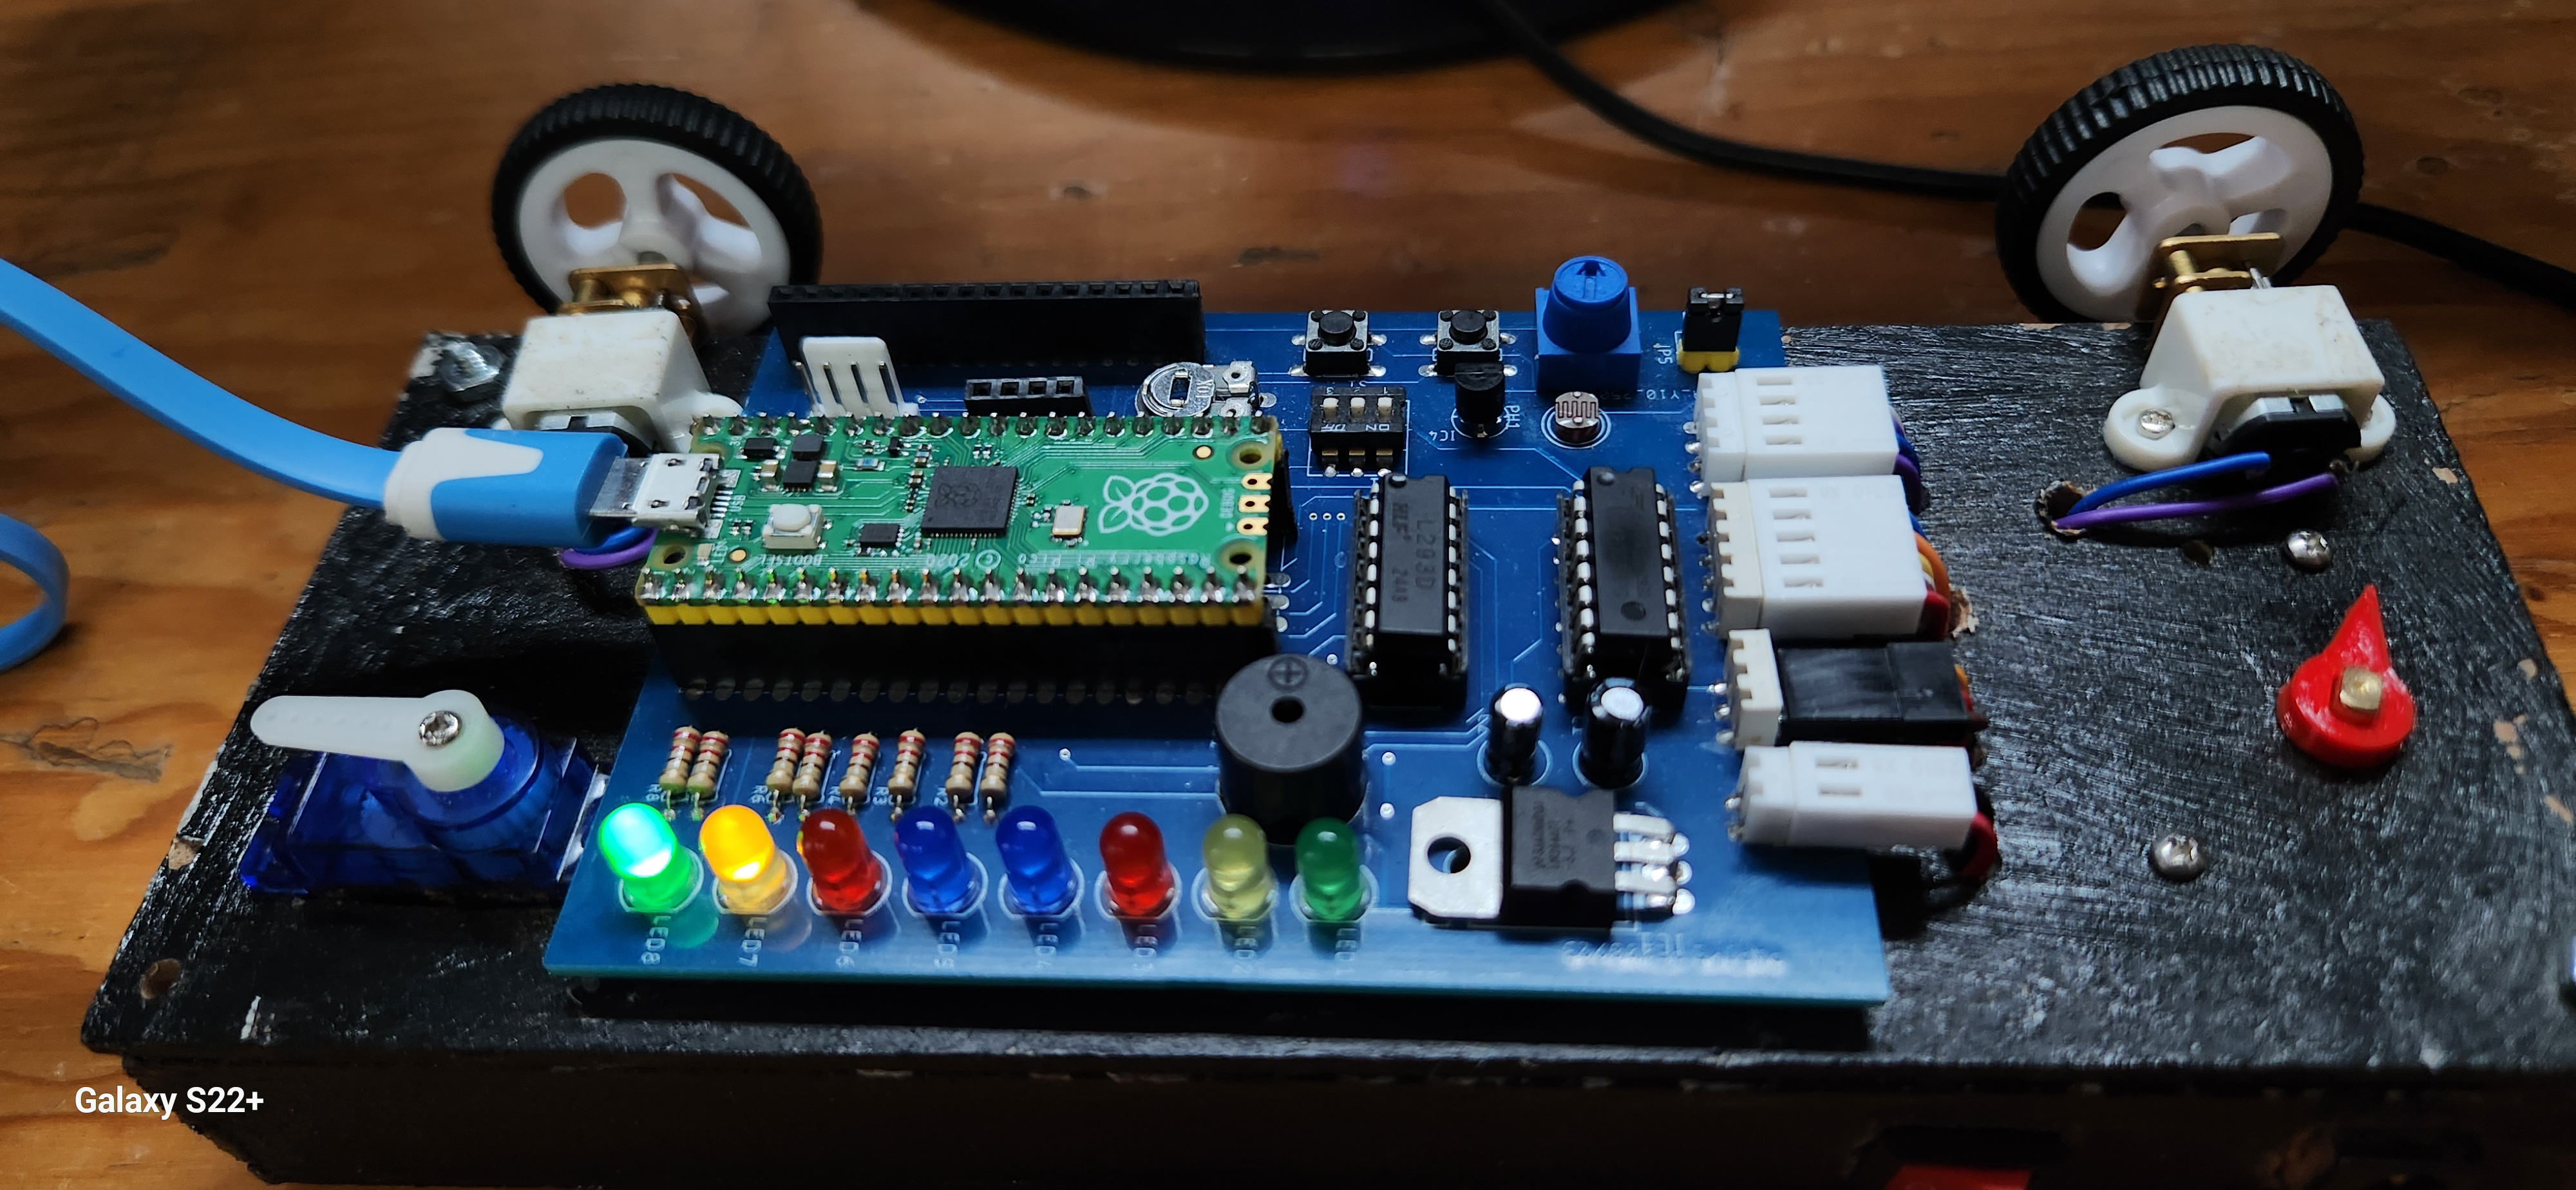
\includegraphics[width=0.8\textwidth]{img/Actividad6/20260325_114747.jpg}
        \caption{Actividad 6: Ambos Leds Encendidos Pt. 1}
    \end{figure}

    \begin{figure}[H]
        \centering
        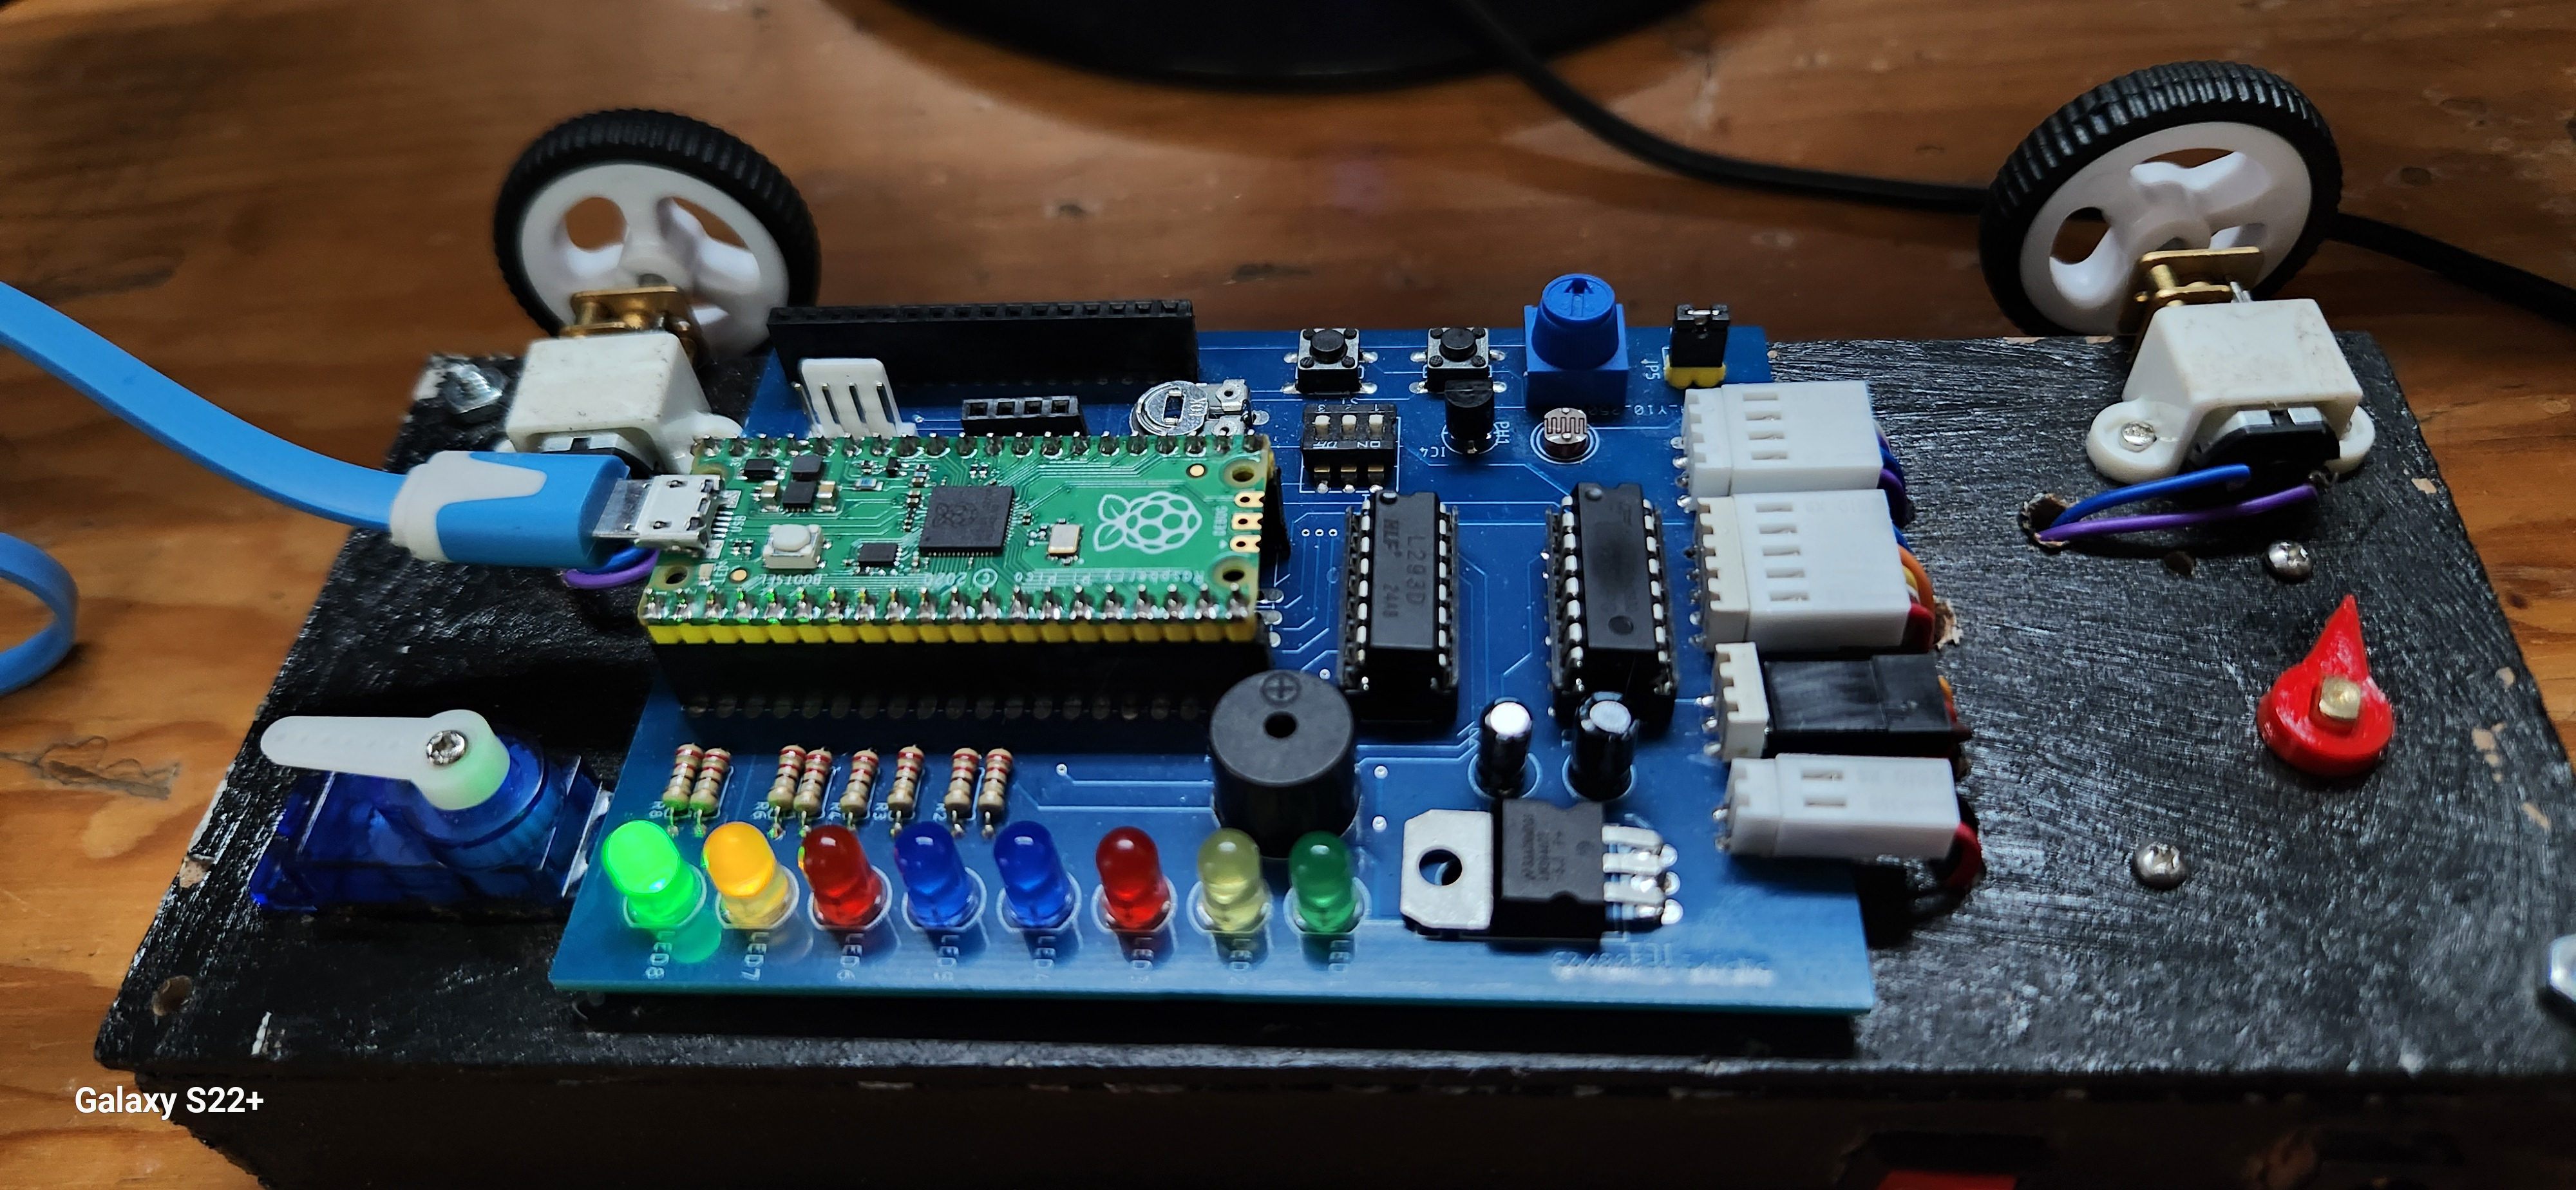
\includegraphics[width=0.8\textwidth]{img/Actividad6/20260325_114758.jpg}
        \caption{Actividad 6: Ambos Leds Encendidos Pt. 2}
    \end{figure}

    \begin{figure}[H]
        \centering
        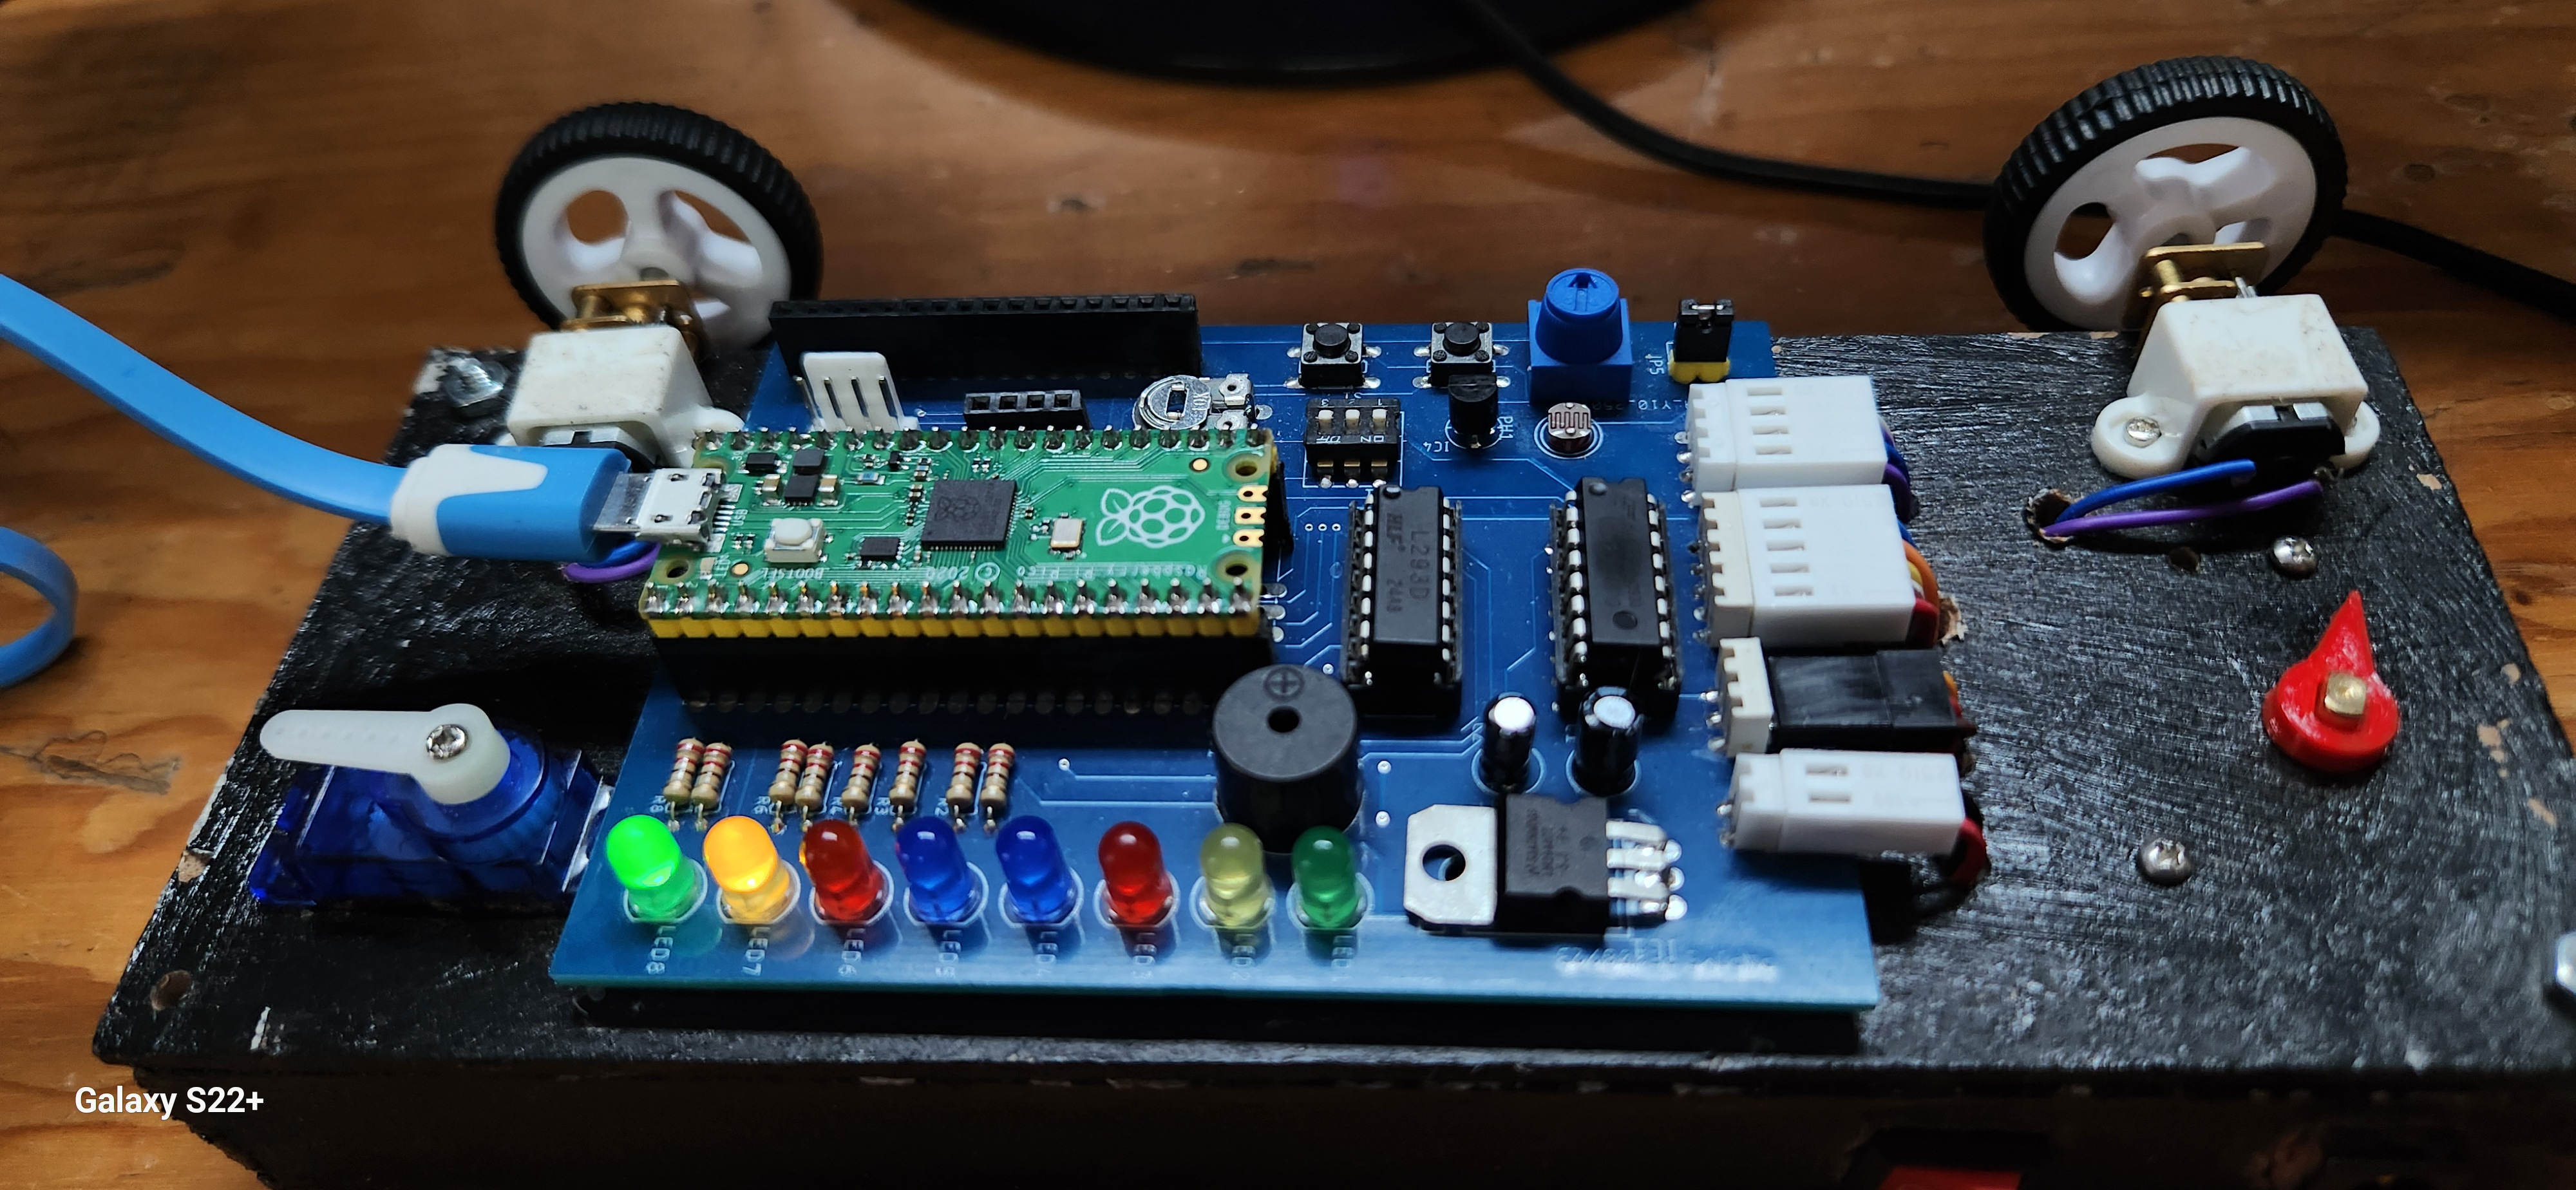
\includegraphics[width=0.8\textwidth]{img/Actividad6/20260325_114755.jpg}
        \caption{Actividad 6: Ambos Leds Encendidos Pt. 2}
    \end{figure}

    A partir de la ejecución del código, se puede observar que ambos LEDs conectados a los pines GPIO0 y GPIO1 se encienden y apagan de manera inversa. Cuando el LED conectado a GPIO0 alcanza su brillo máximo, el LED conectado a GPIO1 está completamente apagado, y viceversa. Este comportamiento confirma que el programa está controlando correctamente los ciclos de trabajo de ambos canales PWM, incrementando uno mientras decrementa el otro. El efecto visual es un ciclo continuo de \texttt{fade} donde un LED se ilumina gradualmente mientras el otro se atenúa, creando un contraste dinámico entre ambos.

    \section*{Actividad 7}

    Realizar las modificaciones necesarias para realizar el control anterior pero ahora a través de la señal analógica proveniente del potenciómetro.

    \begin{figure}[htbp]
        \centering
        \begin{tikzpicture}[>=latex, scale=0.75, transform shape]

            % 1. Dibujar la Raspberry Pi Pico
            \picoboard

            % ==========================================
            % 2. CIRCUITO (Izquierda - Separados y con LEDs hacia abajo)
            % ==========================================

            % --- Rama GP0 (Pin 1 - Verde, la más alejada a la izquierda) ---
            \draw[green!70!black, thick] (P1) -- (-3.0, -0.45);
            \node[above, font=\tiny\sffamily, text=gray] at (-0.8, -0.45) {1};
            \node[above, font=\tiny\sffamily, text=gray] at (-2.8, -0.45) {2};
            
            % Resistencia Superior
            \draw[thick, decoration={zigzag, segment length=3.5mm, amplitude=1.5mm}, decorate] (-3.0, -0.45) -- (-4.5, -0.45);
            \node[above, font=\sffamily] at (-3.75, -0.2) {220$\Omega$};
            \node[above, font=\tiny\sffamily, text=gray] at (-4.7, -0.45) {1};

            % Doblez hacia abajo (Columna X = -5.0)
            \draw[green!70!black, thick] (-4.5, -0.45) -- (-5.0, -0.45) -- (-5.0, -1.2);
            \node[left, font=\tiny\sffamily, text=gray] at (-5.0, -1.0) {1};
            
            % LED 1 (Triángulo apuntando hacia ABAJO)
            \draw[thick] (-5.3, -1.2) -- (-4.7, -1.2) -- (-5.0, -1.8) -- cycle; % Triángulo
            \draw[thick] (-5.3, -1.8) -- (-4.7, -1.8); % Línea base (cátodo)
            
            % Flechas de luz apuntando hacia abajo-izquierda
            \draw[thick, -latex] (-5.4, -1.3) -- (-5.7, -1.7);
            \draw[thick, -latex] (-5.25, -1.45) -- (-5.55, -1.85);
            
            \node[left, font=\tiny\sffamily, text=gray] at (-5.0, -2.0) {2};

            % Conexión a Tierra 1
            \draw[green!70!black, thick] (-5.0, -1.8) -- (-5.0, -2.5);
            \draw[thick] (-5.4, -2.5) -- (-4.6, -2.5);
            \draw[thick] (-5.25, -2.65) -- (-4.75, -2.65);
            \draw[thick] (-5.1, -2.8) -- (-4.9, -2.8);


            % --- Rama GP1 (Pin 2 - Rojo, la más cercana a la Pico) ---
            \draw[red, thick] (P2) -- (-1.5, -0.9);
            \node[above, font=\tiny\sffamily, text=gray] at (-0.8, -0.9) {2};
            \node[above, font=\tiny\sffamily, text=gray] at (-1.3, -0.9) {2};

            % Resistencia Inferior
            \draw[thick, decoration={zigzag, segment length=3.5mm, amplitude=1.5mm}, decorate] (-1.5, -0.9) -- (-3.0, -0.9);
            \node[above, font=\sffamily] at (-2.25, -0.65) {220$\Omega$};
            \node[above, font=\tiny\sffamily, text=gray] at (-3.2, -1.8) {1};
            
            % Doblez hacia abajo (Columna X = -3.5)
            \draw[red, thick] (-3.0, -0.9) -- (-3.5, -0.9) -- (-3.5, -1.2);
            \node[left, font=\tiny\sffamily, text=gray] at (-3.5, -1.05) {1};

            % LED 2 (Triángulo apuntando hacia ABAJO)
            \draw[thick] (-3.8, -1.2) -- (-3.2, -1.2) -- (-3.5, -1.8) -- cycle; % Triángulo
            \draw[thick] (-3.8, -1.8) -- (-3.2, -1.8); % Línea base (cátodo)
            
            % Flechas de luz apuntando hacia abajo-izquierda
            \draw[thick, -latex] (-3.9, -1.3) -- (-4.2, -1.7);
            \draw[thick, -latex] (-3.75, -1.45) -- (-4.05, -1.85);

            \node[left, font=\tiny\sffamily, text=gray] at (-3.5, -2.0) {2};

            % Conexión a Tierra 2
            \draw[green!70!black, thick] (-3.5, -1.8) -- (-3.5, -2.5);
            \draw[thick] (-3.9, -2.5) -- (-3.1, -2.5);
            \draw[thick] (-3.75, -2.65) -- (-3.25, -2.65);
            \draw[thick] (-3.6, -2.8) -- (-3.4, -2.8);

            % ==========================================
            % 3. POTENCIÓMETRO (Centro)
            % ==========================================
            \def\potX{6.5} % Posición X del potenciómetro

            % Cable verde de GP26_A0 (P31) al potenciómetro
            \draw[green!70!black, thick] (P31) -- (6.0, -4.5);
            \fill[green!70!black] (6.0, -4.5) circle (1.5pt); % Nodo
            \draw[->, thick] (6.0, -4.5) -- (6.4, -4.5); % Flecha al zigzag
            \node[font=\tiny\sffamily, text=gray, above] at (6.2, -4.5) {3}; % Etiqueta 3

            % Zigzag del potenciómetro
            \draw[thick, decoration={zigzag, segment length=3.5mm, amplitude=1.5mm}, decorate] (6.5, -3.5) -- (6.5, -5.5);

            % Conexión superior a 3.3V (Cable Rojo)
            \draw[red, thick] (6.5, -3.5) -- (6.5, -2.5);
            \draw[thick] (6.2, -2.5) -- (6.8, -2.5);
            \node[above, font=\sffamily] at (6.5, -2.5) {3.3V};
            \node[left, font=\tiny\sffamily, text=gray] at (6.5, -3.5) {1};

            % Conexión inferior a Tierra (Cable Verde)
            \draw[green!70!black, thick] (6.5, -5.5) -- (6.5, -6.5);
            \draw[thick] (6.2, -6.5) -- (6.8, -6.5);
            \draw[thick] (6.35, -6.6) -- (6.65, -6.6);
            \draw[thick] (6.45, -6.7) -- (6.55, -6.7);
            \node[left, font=\tiny\sffamily, text=gray] at (6.5, -5.5) {2};

            % Etiqueta del potenciómetro
            \node[right, font=\sffamily, align=left] at (6.7, -4.5) {Potenciómetro\\10k$\Omega$};

            % ==========================================
            % 4. OSCILOGRAMAS (Derecha - Desplazados para dar espacio al potenciómetro)
            % ==========================================
            \begin{scope}[scale=0.7, shift={(3.5, 2.5)}]
                \node[anchor=west, font=\sffamily\Large\bfseries] at (9.5, -2.5) {GPIO0};
                
                \begin{scope}[shift={(11.5, -2.5)}]
                    \draw[thick] (0, 0.4) -- ++(0.5, 0); 
                    \foreach \x/\w in {0.5/0.2, 0.9/0.2, 1.3/0.2, 1.7/0.2, 2.1/0.2, 2.5/0.2, 2.9/0.2, 3.3/0.2, 3.7/0.2, 4.1/0.2, 4.5/0.2, 4.9/0.2, 5.3/0.2} {
                        \draw[thick] (\x, 0.4) -- (\x, 0) -- ++(\w, 0) -- ++(0, 0.4) -- ++(0.2, 0);
                    }
                    \draw[thick] (5.9, 0.4) -- ++(0.1, 0);
                \end{scope}

                \node[anchor=west, font=\sffamily\Large\bfseries] at (9.5, -4.5) {GPIO1};
                
                \begin{scope}[shift={(11.5, -4.5)}]
                    \draw[thick] (0, 0) -- ++(1.0, 0); 
                    \foreach \x/\w in {1.0/0.8, 2.8/0.8, 4.6/0.8} {
                        \draw[thick] (\x, 0) -- (\x, 0.4) -- ++(\w, 0) -- ++(0, -0.4) -- ++(1.0, 0);
                    }
                    \draw[thick] (6.4, 0) -- ++(0.1, 0);
                \end{scope}
            \end{scope}

            % ==========================================
            % 5. TÍTULO DE LA FIGURA
            % ==========================================
            \node[font=\sffamily\Large] at (5.0, -11.0) {Figura 6.9. Control PWM por medio de entrada analógica; actividad 7};

        \end{tikzpicture}
    \end{figure}

    \section*{Propuesta de solución}

    Para implementar el control del PWM utilizando la señal analógica proveniente del potenciómetro, es necesario importar el módulo \texttt{ADC} esto para poder leer el valor analógico del potenciómetro, ya que funciona como un convertidor analógico a digital (ADC). Posteriormente se debe de indicar al microcontrolador que el pin 26 se usará para leer una señal analógica, esto se logra creando un objeto de la clase \texttt{ADC} asociado al pin 26. Posteriormente, se establece la frecuencia del PWM para ambos canales en 1 kHz, y se define una variable \texttt{MAX\_DUTY} con el valor máximo de 65535 para controlar el ciclo de trabajo.

    De igual forma qye en el ejercicio anterior, se define la constante \texttt{MAX\_DUTY} con el valor máximo de 65535 para controlar el ciclo de trabajo. Luego, se implementa un bucle infinito que lee continuamente el valor del potenciómetro utilizando el método \texttt{read\_u16()} del objeto ADC. Este método devuelve un valor de 16 bits que representa la posición del potenciómetro, donde 0 corresponde a la posición mínima y 65535 a la posición máxima. Posteriormente, se asigna este valor directamente al canal PWM conectado a GPIO0, mientras que el canal PWM conectado a GPIO1 recibe el valor inverso (calculado como \texttt{MAX\_DUTY - duty}). Esto permite que al girar el potenciómetro en una dirección, un LED se ilumine más mientras el otro se atenúa, y al girarlo en la dirección opuesta, el efecto se invierte. Se introduce un pequeño retardo de 50 milisegundos en cada iteración para que los cambios sean perceptibles visualmente.
     
    \begin{figure}[htbp]
    \centering
    \begin{tikzpicture}[>=latex, scale=0.8, transform shape,
        inicio/.style={ellipse, draw, thick, minimum width=2cm, minimum height=0.8cm, fill=green!20},
        proceso/.style={rectangle, draw, thick, minimum width=3cm, minimum height=0.7cm, fill=blue!10, align=center, font=\footnotesize},
        terminal/.style={rectangle, draw, thick, minimum width=2.5cm, minimum height=0.7cm, fill=orange!10, align=center, font=\footnotesize, rounded corners=5pt},
        flecha/.style={->, thick, rounded corners=2pt} % Esquinas redondeadas para mayor fluidez
    ]
        % --- Bloque de Inicio ---
        \node[inicio] (inicio) at (0, 0) {Inicio};

        % --- Bloque de Configuración ---
        % Se agrupan las configuraciones iniciales
        \node[proceso] (config) at (0, -1.8) {
            Configurar ADC en Pin 26 (Potenciómetro)\\
            Configurar PWM0 en GPIO0\\
            Configurar PWM1 en GPIO1\\
            Frecuencia = 1000 Hz
        };

        % --- Definición de Constantes ---
        \node[proceso] (const) at (0, -3.8) {MAX\_DUTY = 65535};

        % --- Punto de entrada al bucle While True ---
        % Usamos una coordenada vacía como punto de anclaje para el retorno del bucle
        \coordinate (bucle) at (0, -4.8);

        % --- Bloque de Lectura (Terminal/Entrada) ---
        \node[terminal] (lectura) at (0, -5.8) {Leer ADC (read\_u16)\\Guardar en 'lectura\_pot'};

        % --- Bloque de Procesamiento (Cálculos y Escritura) ---
        \node[proceso] (proceso) at (0, -8) {
            Establecer PWM0 = lectura\_pot\\
            Calcular Inverso = MAX\_DUTY - lectura\_pot\\
            Establecer PWM1 = Inverso
        };

        % --- Bloque de Espera ---
        \node[proceso] (espera) at (0, -10) {Esperar 0.05 segundos};

        % ================= RUTAS Y FLECHAS =================
        
        % Flujo secuencial inicial
        \draw[flecha] (inicio) -- (config);
        \draw[flecha] (config) -- (const);
        
        % Entrada al bucle
        \draw[thick] (const) -- (bucle); % Línea continua hasta el punto de anclaje
        \draw[flecha] (bucle) -- (lectura);
        
        % Flujo dentro del bucle
        \draw[flecha] (lectura) -- (proceso);
        \draw[flecha] (proceso) -- (espera);
        
        % --- Retorno del Bucle While True ---
        % Sale de 'espera', va a la izquierda y sube hasta el punto 'bucle'
        \draw[flecha] (espera.south) -- ++(0,-0.8) -| (-4, -4.8) -- (bucle);

    \end{tikzpicture}
    \caption{Diagrama de flujo: Control de LEDs directo e inverso mediante Potenciómetro (ADC) - Actividad 7}
\end{figure}

    \section*{Desarrollo}

    \lstinputlisting[language={[LAB]Python}, caption=Código de la Actividad 7,basicstyle=\ttfamily\scriptsize]{Code/Act7.py}

    \subsection*{Análisis de resultados}

    \begin{figure}[H]
        \centering
        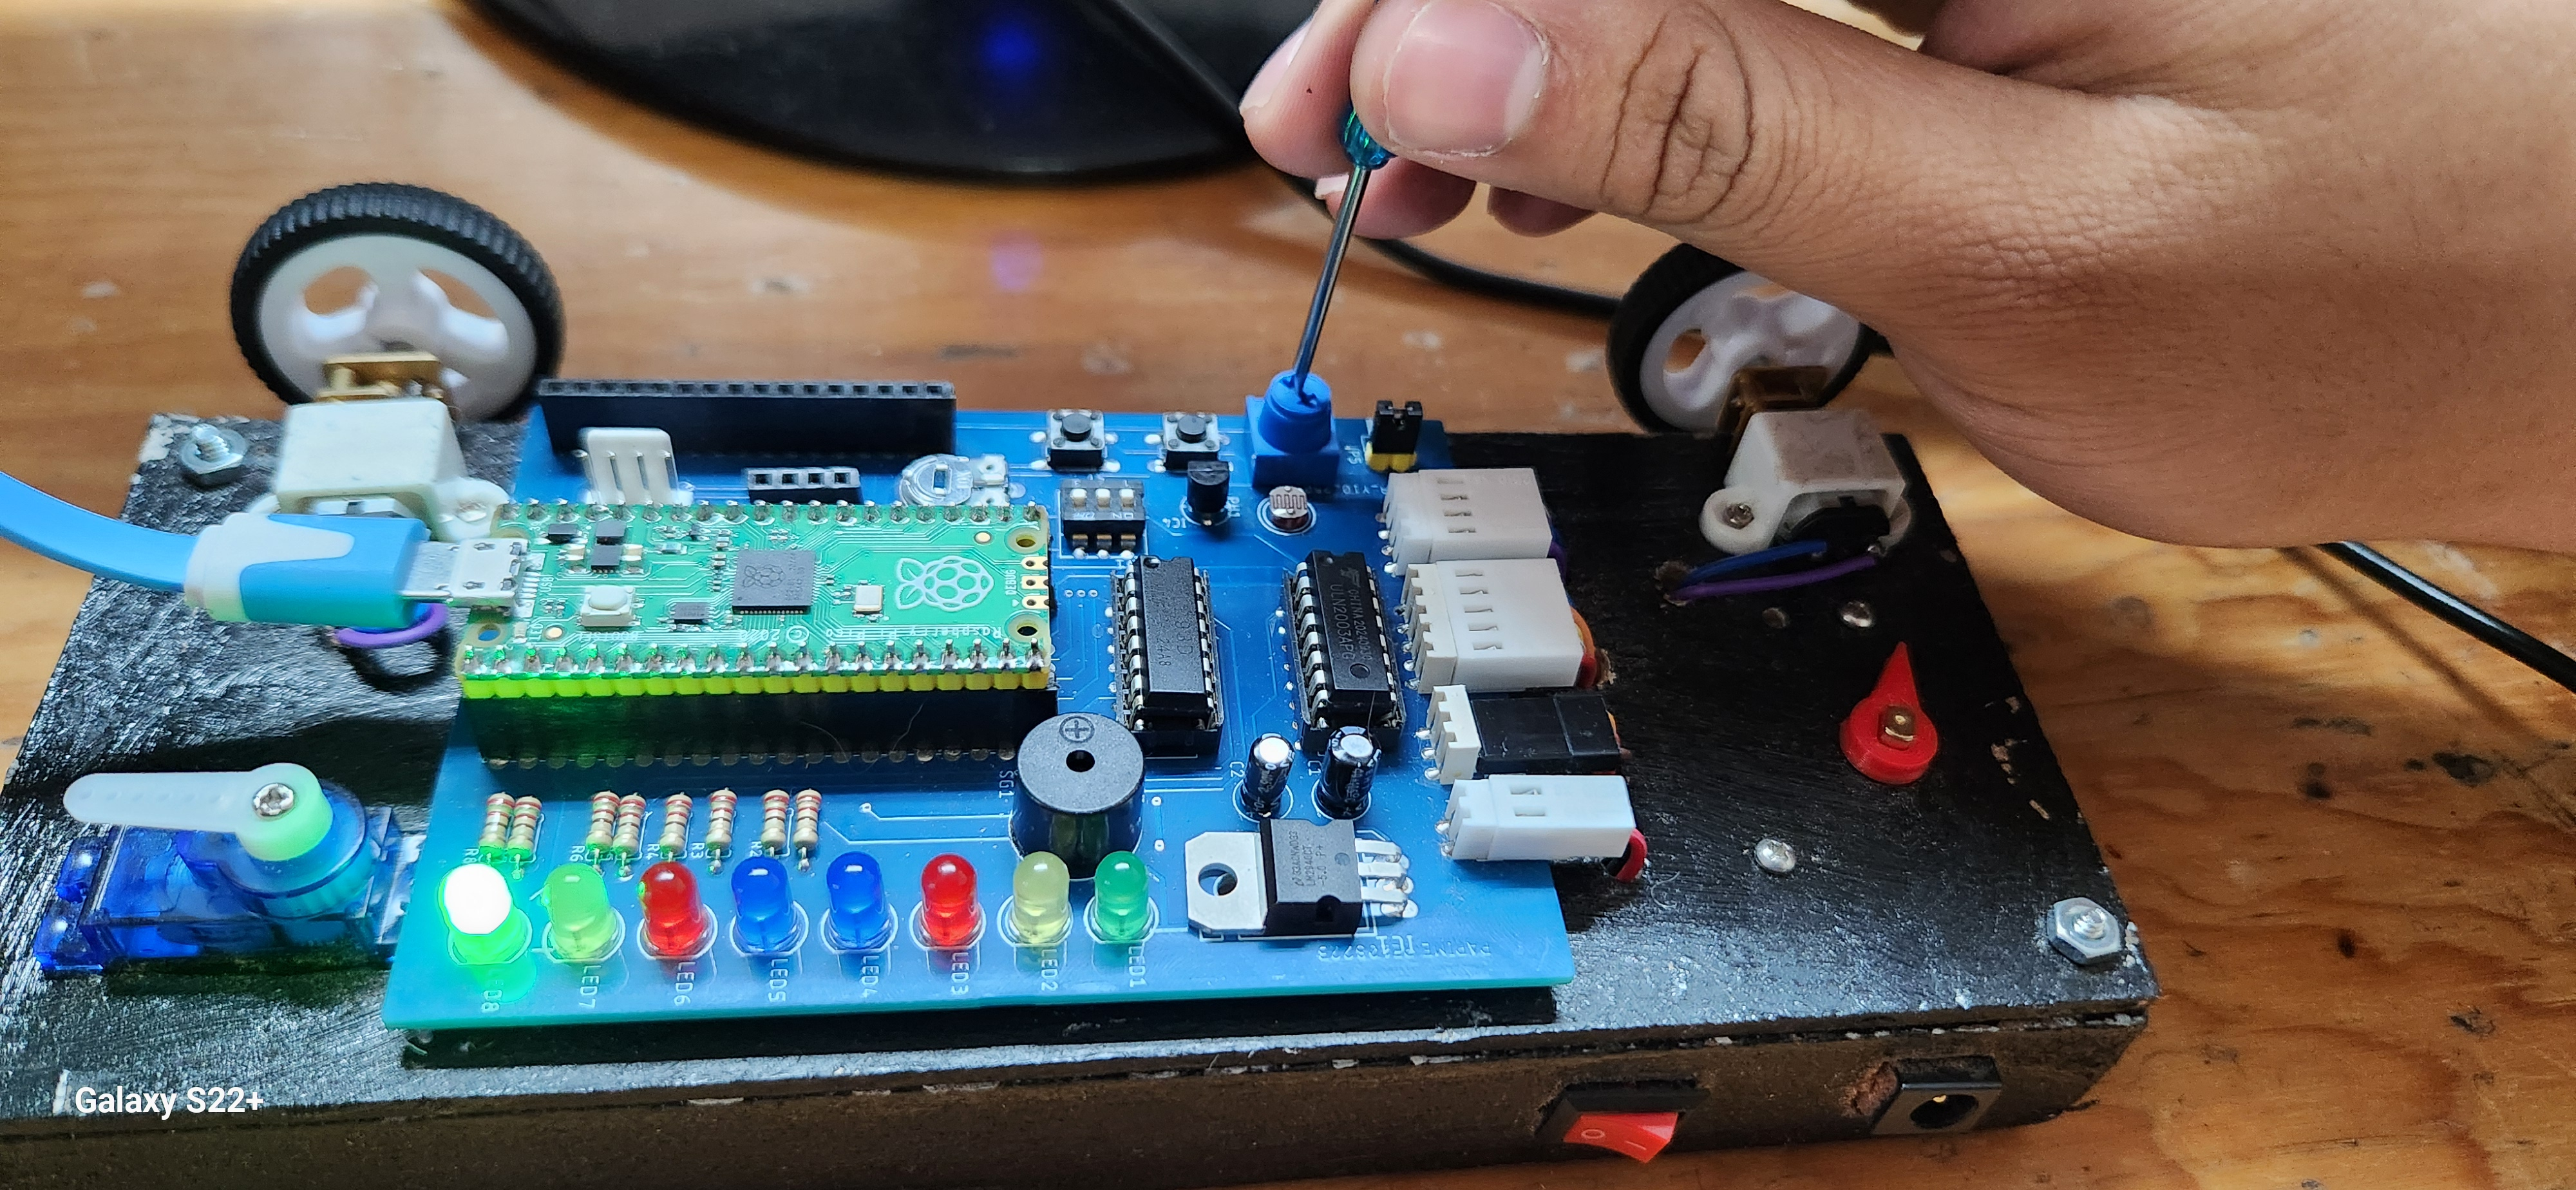
\includegraphics[width=0.8\textwidth]{img/Actividad7/20260325_114705.jpg}
        \caption{Actividad 7: Potenciómetro con un valor bajo}
    \end{figure}

    \begin{figure}[H]
        \centering
        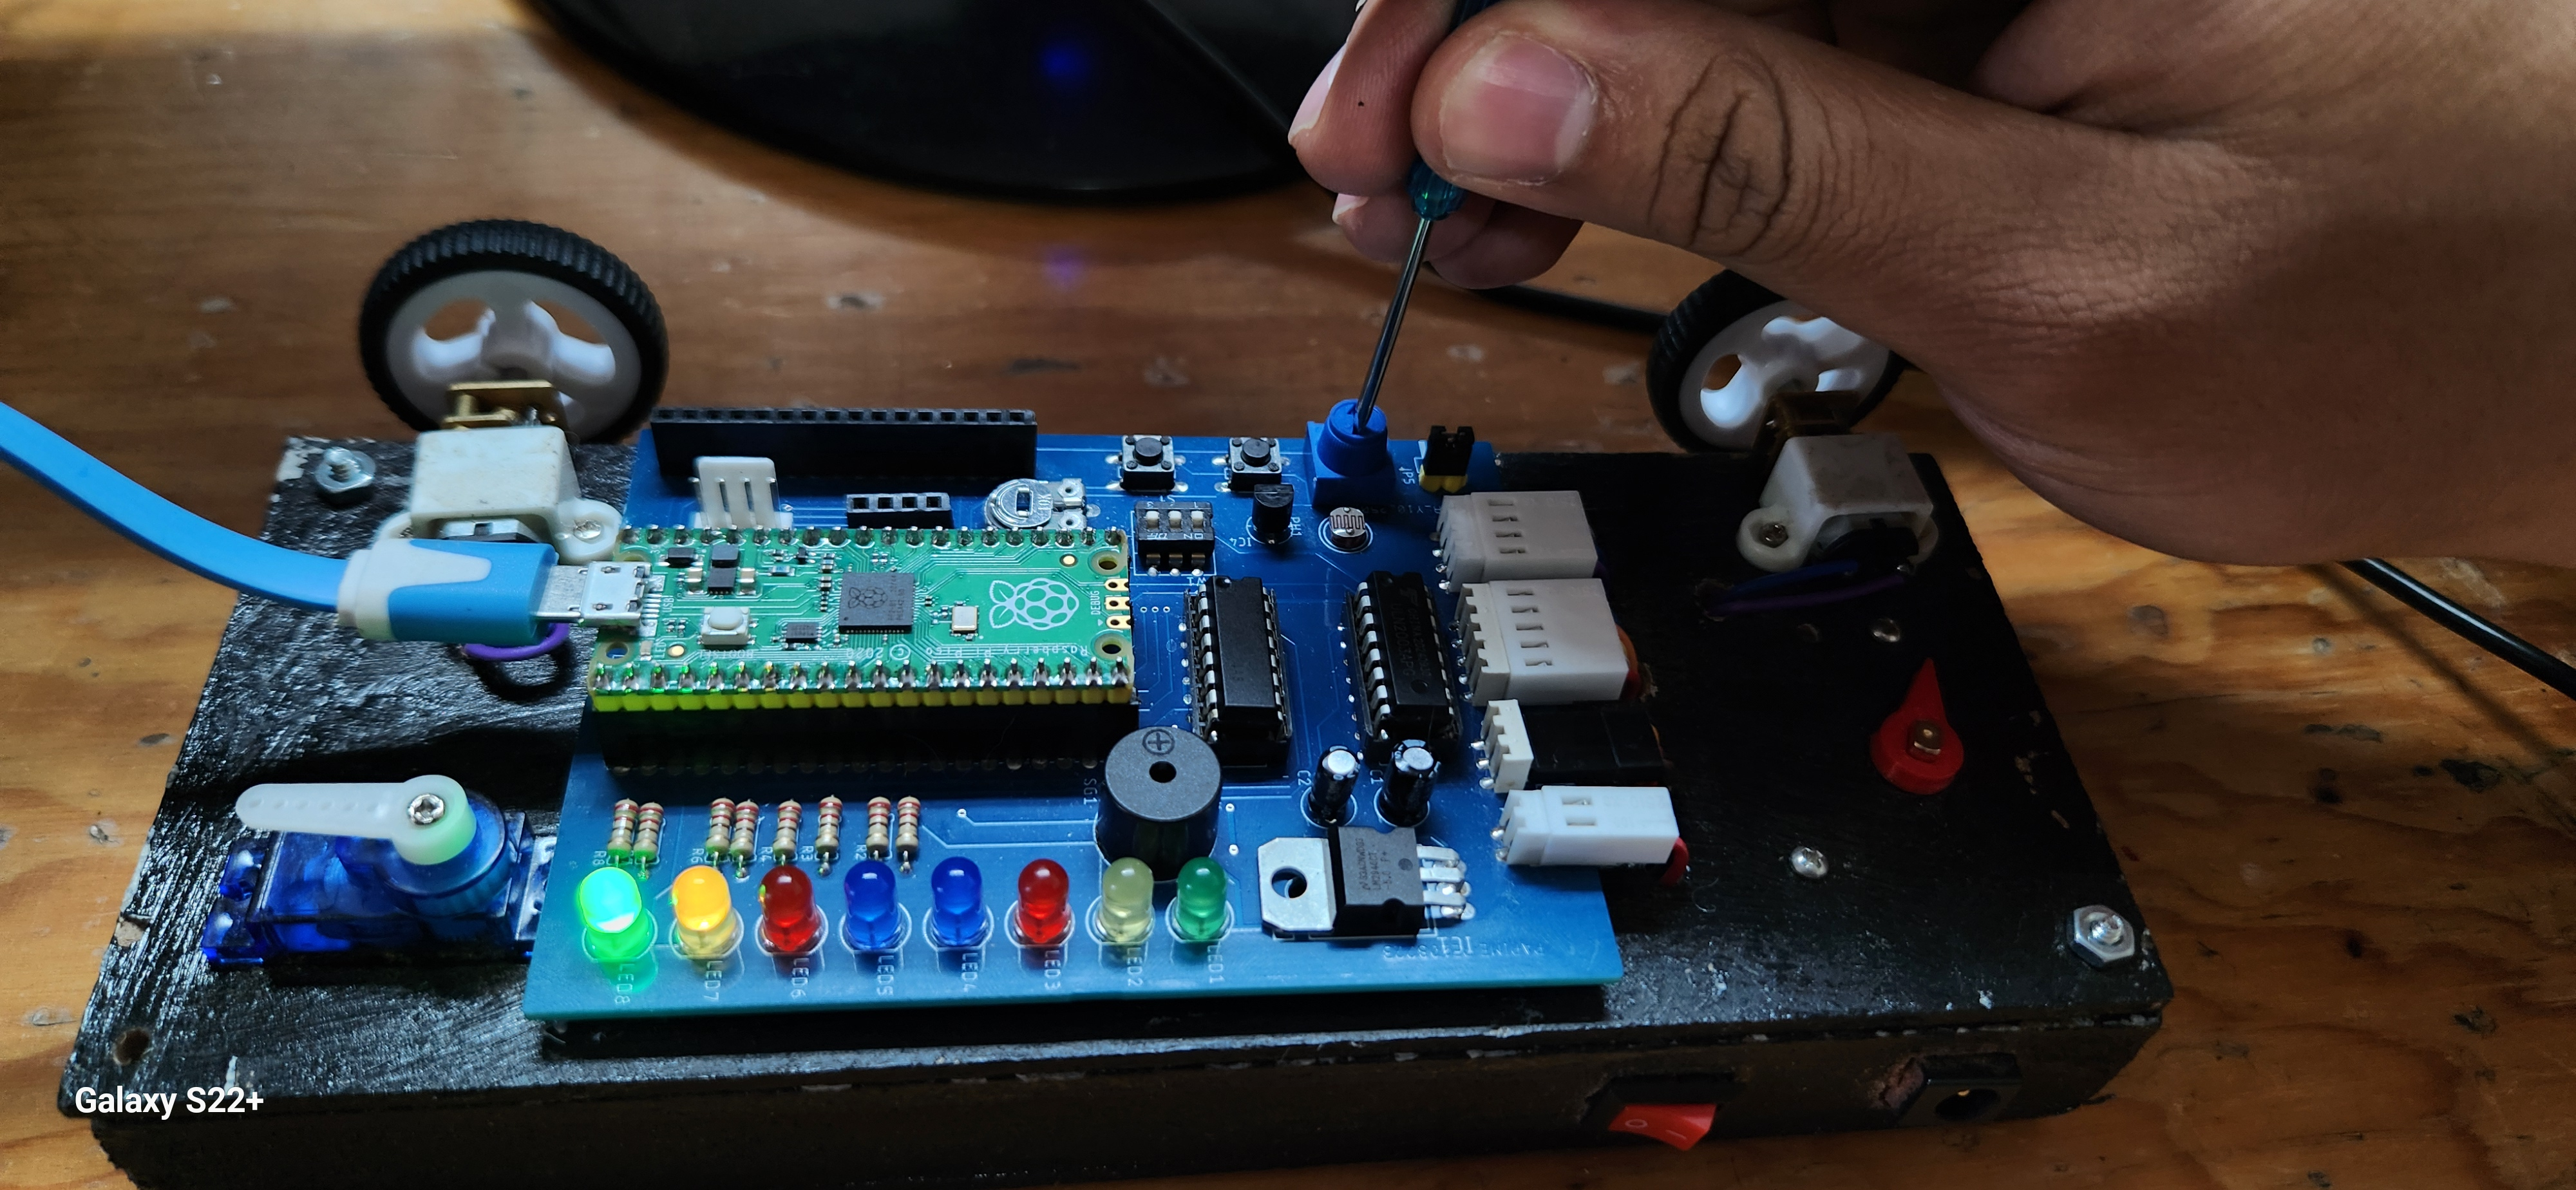
\includegraphics[width=0.8\textwidth]{img/Actividad7/20260325_114716.jpg}
        \caption{Actividad 7: Potenciómetro con un valor medio}
    \end{figure}

    \begin{figure}[H]
        \centering
        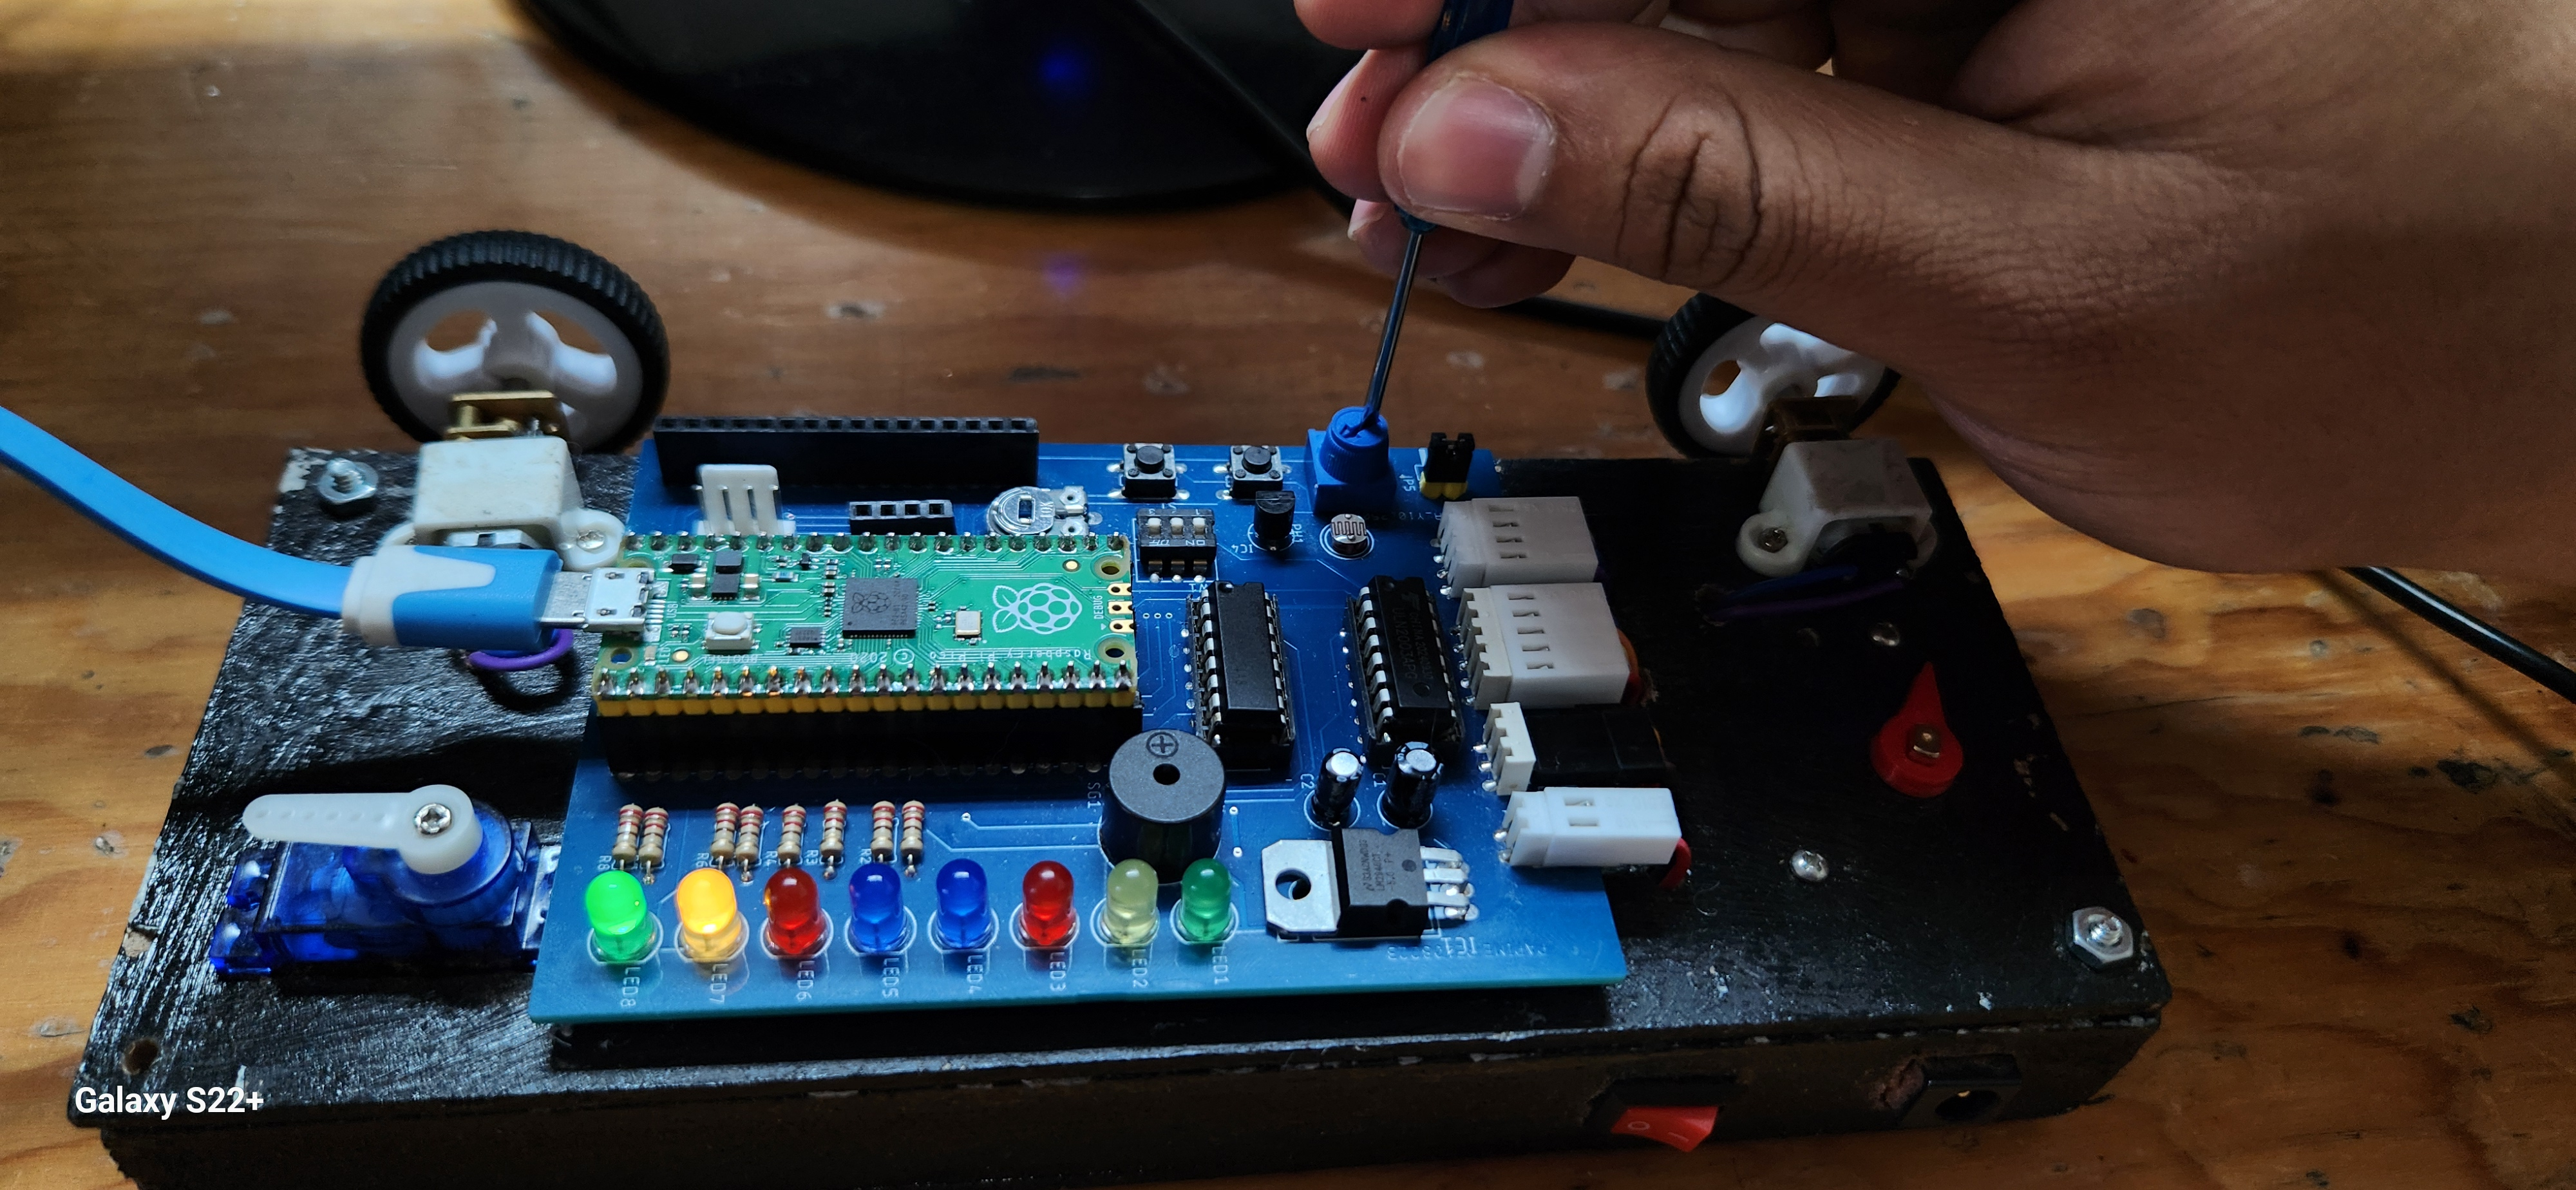
\includegraphics[width=0.8\textwidth]{img/Actividad7/20260325_114719.jpg}
        \caption{Actividad 7: Potenciómetro con un valor alto}
    \end{figure}

    Al cargar el programa desarrollado para esta actividad, se puede observar que al girar el potenciómetro, el brillo de los LEDs conectados a \texttt{GPIO0} y \texttt{GPIO1} cambia de manera inversa. Cuando el potenciómetro está en su posición mínima, el LED conectado a \texttt{GPIO0} está completamente apagado mientras que el LED conectado a \texttt{GPIO1} está en su brillo máximo. A medida que se gira el potenciómetro hacia la posición media, el LED de \texttt{GPIO0} comienza a iluminarse gradualmente mientras que el LED de \texttt{GPIO1} se atenúa. Finalmente, al girar el potenciómetro hacia su posición máxima, el LED de \texttt{GPIO0} alcanza su brillo máximo y el LED de \texttt{GPIO1} se apaga completamente. Es a partir de este comportamiento  que se puede confirmar que la lectura del ADC del potenciómetro está controlando correctamente los ciclos de trabajo de ambos canales PWM, creando un efecto dinámico donde un LED se ilumina mientras el otro se atenúa en función de la posición del potenciómetro.

    \newpage
    \section{Conclusiones:}

    \begin{itemize}
        \item \textbf{Espinoza Matamoros Percival Ulises:} Por medio de las diferentes actividades realizadas en está práctica pude comprender y conocer el funcionamiento de los convertidores analógico a digital (ADC) para diversas aplicaciones como procesar señales analógicas provenientes de sensores, como el potenciómetro y el fotoresistor, de forma que para procesar esta señales por medio del microtrolador es necesario realizar las conversiones necesarias para poder interpretar correctamente la información que se obtiene de estos sensores, esto se logra por medio de la clase \texttt{ADC} en MicroPython. De igual forma, también pude comprender el funcionamiento de los módulos PWM y cómo controlar el ciclo de trabajo para lograr efectos visuales como el  efecto de \texttt{fade} en los LEDs, así como la importancia de configurar correctamente los pines y establecer frecuencias adecuadas para obtener resultados óptimos.
        

        \item \textbf{Flores Colin Victor Jaziel:}
        El desarrollo de esta práctica me permitió comprender de mejor manera la adquisición y procesamiento de señales analógicas mediante el convertidor analógico-digital (ADC) del RP2040, así como la generación de señales digitales mediante modulación por ancho de pulso (PWM). A través de las actividades realizadas, se exploraron diferentes configuraciones del ADC: el uso del canal 0 (GPIO26) para leer un potenciómetro, el canal 1 (GPIO27) para una fotoresistencia en configuración de divisor de voltaje, y el canal 4 interno para acceder al sensor de temperatura del chip y para cada caso se aplicaron las ecuaciones de transferencia correspondientes para escalar los valores digitales de 16 bits a unidades como voltios o grados Celsius para interpretar correctamente las magnitudes físicas.

        Asimismo, se implementó un sistema de control basado en umbrales utilizando la fotoresistencia, donde el registro dinámico de valores máximos y mínimos permitió establecer puntos de referencia adaptativos para activar una salida digital y además se generaron efectos visuales con los leds mediante señales PWM en los pines GPIO0 y GPIO1, variando el ciclo de trabajo para lograr transiciones suaves de intensidad luminosa (efecto \texttt{fade}) y comportamientos complementarios entre dos LEDs. Todas estas actividades me ayudaron a entender la importancia del microcontrolador para interactuar con el mundo físico, combinando sensores analógicos, actuadores digitales y técnicas de procesamiento de señales en aplicaciones de automatización y control.

        \item \textbf{Lara Hernandez Angel Husiel:}

        Implementar la conversión analógico-digital mediante el módulo ADC del RP2040 para leer señales provenientes del potenciómetro, la fotoresistencia y el sensor de temperatura TMP36 me sirvió mucho para entender cómo el microcontrolador traduce magnitudes físicas continuas a valores discretos de 16 bits que pueden ser procesados y escalados al voltaje de referencia del sistema. También vi que configurar los canales ADC en los pines GPIO26, GPIO27 y GPIO28, así como emplear el canal 4 para acceder al sensor de temperatura interno, permite capturar múltiples señales de forma simultánea aplicando las ecuaciones de transferencia específicas de cada sensor para obtener unidades de ingeniería como voltios, grados Celsius o comparaciones lógicas con umbrales de referencia. Además, controlar el ciclo de trabajo de las señales PWM en los pines GPIO0 y GPIO1 a frecuencias fijas de 1 kHz posibilita generar efectos visuales como el fade progresivo en LEDs variando el duty cycle de 0 a 65535, e incluso sincronizar dos salidas con valores inversos para producir comportamientos complementarios. 

    \end{itemize}

    \newpage

    % Impresión Referencias
    \nocite{*}
    \printbibliography[heading=bibintoc, title={Referencias}]
\end{document}